% Multi-Object Tracking for Sports Analytics (Player and Ball Tracking)
% IEEE conference format (IEEEtran).
%
% Compile:  pdflatex FINAL_REPORT.tex   (run twice so references resolve)
%           or upload FINAL_REPORT_IEEE_overleaf.zip to Overleaf.
%
% This file is GENERATED by scripts/make_latex_report.py from
% docs/latex/FINAL_REPORT.template.tex and results/metrics/. Edit the template
% (text) or re-run the experiments (numbers), then run the script again.
% Figures are expected in the folder figures/ next to this file.
% ----------------------------------------------------------------------------
\documentclass[conference]{IEEEtran}
\IEEEoverridecommandlockouts
\usepackage[T1]{fontenc}
\usepackage{cite}
\usepackage{amsmath,amssymb}
\usepackage{graphicx}
\usepackage{booktabs}
\usepackage{array}
\usepackage{adjustbox}
\usepackage{url}
% --- Float placement -------------------------------------------------------
% dblfloatfix keeps figure and figure* in the right order and lets wide
% floats go at the top or bottom of a page. The settings below let LaTeX put
% more floats on a text page, so figures stay next to the text that cites
% them and do not pile up at the end of the paper.
\usepackage{dblfloatfix}
\usepackage{placeins}  % \FloatBarrier
\renewcommand{\topfraction}{0.85}
\renewcommand{\bottomfraction}{0.6}
\renewcommand{\textfraction}{0.1}
\renewcommand{\floatpagefraction}{0.75}
\renewcommand{\dbltopfraction}{0.85}
\renewcommand{\dblfloatpagefraction}{0.75}
\setcounter{topnumber}{3}
\setcounter{bottomnumber}{2}
\setcounter{totalnumber}{5}
\setcounter{dbltopnumber}{3}
\graphicspath{{figures/}}

\begin{document}

\title{Multi-Object Tracking for Sports Analytics:\\
Player and Ball Tracking with YOLO11n, ByteTrack, a Kalman Filter and Motion-Based Ball Flights}

\author{
\IEEEauthorblockN{Ravva Siddhartha}
\IEEEauthorblockA{\textit{Dept. of Computer Science}\\
\textit{and Engineering}\\
\textit{Amrita School of Computing}\\
Amrita Vishwa Vidyapeetham\\
Bengaluru, India\\
\texttt{bl.en.u4cse23246@bl.students.amrita.edu}}
\and
\IEEEauthorblockN{Pulapa Yaswanth Kumar}
\IEEEauthorblockA{\textit{Dept. of Computer Science}\\
\textit{and Engineering}\\
\textit{Amrita School of Computing}\\
Amrita Vishwa Vidyapeetham\\
Bengaluru, India\\
\texttt{bl.en.u4cse23245@bl.students.amrita.edu}}
\and
\IEEEauthorblockN{Tripty Singh}
\IEEEauthorblockA{\textit{Dept. of Computer Science}\\
\textit{and Engineering}\\
\textit{Amrita School of Computing}\\
Amrita Vishwa Vidyapeetham\\
Bengaluru, India\\
\texttt{tripty\_singh@blr.amrita.edu}}
}

\maketitle

\begin{abstract}
Sports analytics needs two signals from a match video: where each player is,
under an identity that does not change, and where the ball is. This work builds
and evaluates a tracking-by-detection system for soccer that runs on an ordinary
laptop CPU with pretrained models only. A COCO-pretrained YOLO11n network
detects people and the ball in one pass per frame. ByteTrack links the player
detections into persistent tracks, and a constant-velocity Kalman filter follows
the ball, filling short detection gaps with positions that are always marked as
predictions. A motion stage extends the ball tracker to shots, when the blurred
ball is invisible to the detector. We compare ByteTrack against SORT and OC-SORT
on identical cached detections over six test sequences from SportsMOT and
UVY-Track, and evaluate the ball on 13 sequences from UVY-Track and
InFactory. On SportsMOT, ByteTrack makes the fewest identity switches
(51 against 60 for SORT and 106 for
OC-SORT), whereas SORT reaches the highest HOTA (65.9 against
62.6). On the partially labelled UVY-Track clips ByteTrack has the
best OWTA (56.8). Against published SportsMOT results, the gap to
the best tracker (Deep-EIoU, HOTA 77.2) lies almost entirely in
detection accuracy, not in association. For the ball, the tracker improves F1 on
the held-out InFactory clips (51.0 against 47.1) but
not on UVY-Track, and its clearest benefit is a far more continuous ball track.
\end{abstract}

\begin{IEEEkeywords}
multi-object tracking, sports analytics, soccer, ball tracking, YOLO, ByteTrack,
Kalman filter, HOTA
\end{IEEEkeywords}

% =============================================================================
\section{Introduction}
% =============================================================================
Coaches, analysts and broadcasters increasingly rely on automatic analysis of
match footage: distance covered, heatmaps, passing networks and team shape are
all computed from player and ball positions over time. Obtaining those
positions from a single camera is a multi-object tracking (MOT) problem, and
soccer makes it harder than most. Team-mates wear identical kits, so appearance
says little about identity. Players accelerate, turn and occlude one another in
duels and set pieces. The camera pans and zooms, mixing its own motion into the
image. The ball is the hardest object of all: it covers only a few pixels, is
blurred when struck, and is frequently hidden behind players.

Most published sports trackers are trained on the target benchmark and run on
GPUs. We study the other end of the spectrum: what classic trackers achieve with
a small, generic detector on a CPU, which is the realistic setting for a
low-cost system. Players and the ball are treated as separate problems. Players
are many similar targets and need global assignment, so they are tracked with
ByteTrack~\cite{bytetrack}. The ball is a single, often missed target, so it gets
a dedicated Kalman-filter tracker~\cite{kalman} that decides which candidate, if
any, is the ball and reports clearly when a position is predicted rather than
observed.

The contributions of this work are:
\begin{itemize}
\item an end-to-end pipeline that turns a soccer video into an annotated video, a
per-frame tracking table and a run summary, in which every predicted ball
position is labelled as such;
\item a controlled comparison of ByteTrack, SORT~\cite{sort} and
OC-SORT~\cite{ocsort}, in which all three replay the same detections and receive
the same tuning budget on a sequence that is never used for testing;
\item an evaluation on three public datasets with different annotation schemes,
including a study of how partial and carried-forward labels distort
false-positive-based metrics;
\item a placement of the results against published SportsMOT
results~\cite{sportsmot,deepeiou,diffmot}, showing where the remaining gap lies.
\end{itemize}

% =============================================================================
\section{Related Work}
% =============================================================================
\textbf{Tracking by detection.} SORT~\cite{sort} predicts every track with a
Kalman filter~\cite{kalman} and matches predictions to detections by box overlap,
which made it a fast and strong reference design. ByteTrack~\cite{bytetrack}
observed that dropping low-confidence detections discards real objects that are
merely occluded or blurred, and added a second matching stage for them.
OC-SORT~\cite{ocsort} kept the SORT structure but corrects the error the filter
accumulates while a target is unobserved. Later sports trackers add appearance
cues and better motion models: MixSort~\cite{sportsmot} attaches an appearance
association model, Deep-EIoU~\cite{deepeiou} combines an expanding IoU with deep
re-identification features, and DiffMOT~\cite{diffmot} predicts non-linear motion
with a diffusion model.

\textbf{Sports benchmarks.} SportsMOT~\cite{sportsmot} provides broadcast
basketball, volleyball and football clips with every player annotated, and
reports that association, rather than detection, is the main difficulty in
sports scenes. UVY-Track~\cite{uvy} collects user-generated sports videos, a less
controlled setting with hand-held cameras and crowds.

\textbf{Ball tracking.} Early work exploited the ball's trajectory to separate it
from look-alike candidates~\cite{yu2006}, an idea that motion models still use.
The InFactory dataset~\cite{infactory} targets the small, blurred broadcast ball
and labels frames in which the ball is not visible.

\textbf{Detectors and metrics.} This work uses the COCO-pretrained~\cite{coco}
YOLO11 nano model~\cite{yolo11}. Tracking quality is reported with
CLEAR-MOT~\cite{clear}, IDF1~\cite{idf1}, HOTA~\cite{hota}, which separates
detection from association, and OWTA~\cite{owta}, which suits data where not
every object is labelled.

\textbf{Related work at Amrita Vishwa Vidyapeetham, Bengaluru.} YOLO detectors
have been applied to online exam proctoring~\cite{singh2024proctor}, classroom
attentiveness monitoring~\cite{nair2023attentive} and a low-cost perception
framework for autonomous driving~\cite{gopikiran2025driving}. Detection combined
with tracking has been used for multiple pedestrians~\cite{kumar2023pedestrian},
the task closest to player tracking, and for small, fast animals with YOLOv8 and
DeepSORT~\cite{peri2023animals}. Moving-object detection in surveillance
video~\cite{aarthi2016moving} relates to the motion stage used here for the ball
in flight.

% =============================================================================
\section{Methodology}
% =============================================================================
\begin{figure*}[!t]
\centering
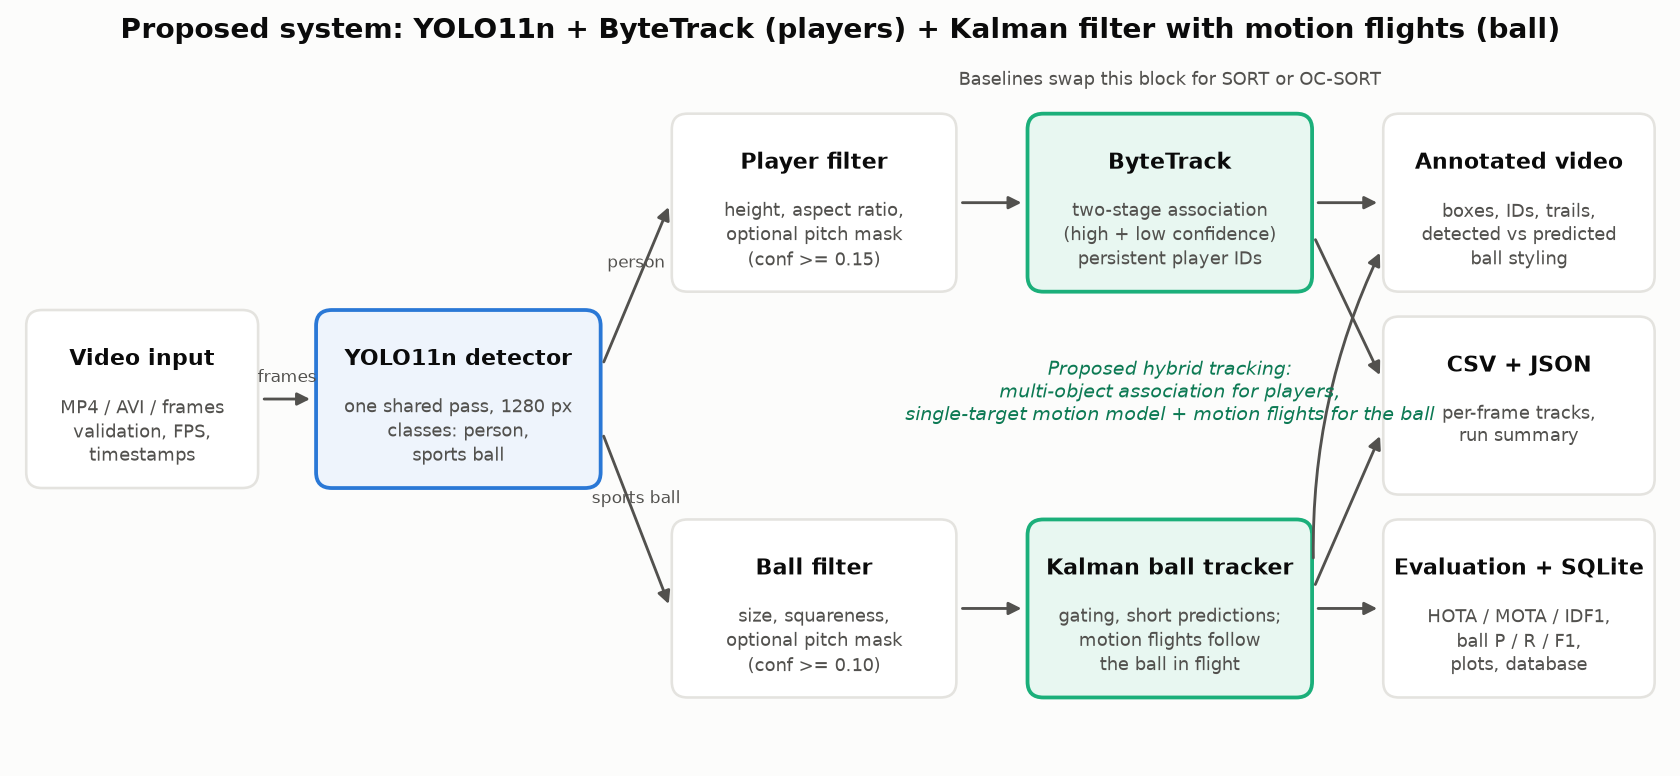
\includegraphics[width=0.9\textwidth]{fig_architecture.png}
\caption{System architecture. A single YOLO11n pass per frame feeds both the
player branch (filter, ByteTrack) and the ball branch (filter, motion stage,
Kalman tracker). The baselines replace only the ByteTrack block.}
\label{fig:architecture}
\end{figure*}

\subsection{System overview}
Fig.~\ref{fig:architecture} shows the pipeline. Each decoded frame goes once
through the detector, which reports the COCO classes \emph{person} and
\emph{sports ball}. Simple geometric filters discard implausible boxes. Player
boxes are passed to the multi-object tracker and ball candidates to the ball
tracker. The tracked objects are drawn onto the frame and written to a
comma-separated file, and a JSON summary is produced at the end of the run.

\subsection{Datasets}
\label{sec:datasets}
Three public datasets are used (Table~\ref{tab:datasets}), each read by its own
loader; annotations from different datasets are never mixed. In total
4{,}850 frames are evaluated (1{,}831 SportsMOT, 1{,}569
UVY-Track, 1{,}450 InFactory); Table~\ref{tab:sequences} lists them. Only
the sequences actually used were downloaded, by reading the remote archives
selectively.

\begin{table*}[!t]
\caption{Datasets and their role in this work}
\label{tab:datasets}
\centering
\footnotesize
\begin{tabular}{@{}p{2.5cm}p{4.3cm}p{5.0cm}p{4.4cm}@{}}
\toprule
 & SportsMOT~\cite{sportsmot} & UVY-Track~\cite{uvy} & InFactory~\cite{infactory} \\
\midrule
Footage & Professional broadcast & User-generated online video & Professional soccer broadcast \\
Annotation format & MOT Challenge text & MOT-style text with class and visibility & YOLO text per frame \\
Annotated objects & Athletes on the field only & Players, goalkeepers, referees, ball & Ball only, plus ``ball not visible'' frames \\
Identities & Players & People and ball & None \\
Used for & Player tracking (tuning and test) & Player tracking and ball (test) & Ball detection (test) \\
\bottomrule
\end{tabular}
\end{table*}

\begin{table}[!htb]
\caption{Evaluated sequences (Ball fr.: frames scored for the ball)}
\label{tab:sequences}
\centering
\footnotesize
\begin{adjustbox}{max width=\columnwidth}
\begin{tabular}{@{}llcrrr@{}}
\toprule
Dataset & Sequence & Role & Frames & Tracks & Ball fr. \\
\midrule
SportsMOT & \texttt{v\_2QhNRucNC7E\_c017} & dev & 450 & 21 & -- \\
SportsMOT & \texttt{v\_dw7LOz17Omg\_c067} & test & 450 & 22 & -- \\
SportsMOT & \texttt{v\_G-vNjfx1GGc\_c008} & test & 480 & 20 & -- \\
SportsMOT & \texttt{v\_i2\_L4qquVg0\_c007} & test & 451 & 21 & -- \\
UVY-Track & \texttt{soccer\_V04} & test & 219 & 19 & 168 \\
UVY-Track & \texttt{soccer\_V01} & test & 750 & 6 & 494 \\
UVY-Track & \texttt{soccer\_V03} & test & 600 & 5 & 371 \\
InFactory & 10 clips & test & 1{,}450 & -- & 884 \\
\bottomrule
\end{tabular}
\end{adjustbox}
\end{table}

One SportsMOT sequence (\texttt{v\_2QhNRucNC7E\_c017}) is used only to choose
tracker parameters. It comes from a different match than every test sequence and
never enters a test average. Nothing is tuned on UVY-Track or InFactory.

Three properties of the labels shape the evaluation. First, SportsMOT annotates
only the athletes, so referees, coaches and staff found by a generic
\emph{person} detector count as false positives. Second, UVY-Track labels only
some of the people: in the fan-filmed penalty clips just the four to six people
involved in the kick are boxed, while many visible photographers and officials
are not. Third, UVY-Track never marks the ball as absent, and its ball rows with
visibility~0 are not ball positions: inspecting them shows boxes left on empty
grass while the ball is elsewhere, i.e.\ positions carried forward by the
annotation tool. We therefore score a UVY-Track frame for the ball only when it
has a ball box with visibility above zero (1{,}033 frames). This removes
485 frames with carried-forward boxes and 51 frames with no
ball row, such as a shot in flight that was left unlabelled. False alarms on
ball-free frames are measured on InFactory, which labels such frames explicitly.

\subsection{Detection and filtering}
YOLO11n, a network of about 2.6 million parameters, runs at an input size of
1280 pixels. Person boxes are kept from confidence 0.15 and ball boxes from
0.10; these deliberately low thresholds leave the decision of what to trust to
the trackers. A player box must be between 12 pixels and 60\% of the frame
tall, with a height-to-width ratio between 0.8 and 6. A ball box must be 2 to 80
pixels wide and roughly square. Serving both classes from one network pass
halves the detection cost.

\subsection{Player tracking}
The three trackers share a common loop: predict every track with a Kalman
filter, build an intersection-over-union (IoU) cost matrix between predicted and
detected boxes, solve the assignment, update the matched tracks, open tracks
for unmatched detections and close tracks that stay unmatched too long. They
differ in their use of detection confidence. SORT matches in a single stage.
OC-SORT considers only confident detections and re-corrects the filter after an
occlusion. ByteTrack first matches the confident detections and then offers the
remaining tracks the low-confidence ones.

We propose ByteTrack for players because occlusion and motion blur, both
frequent in soccer, lower a detector's confidence without removing the player.
Keeping such tracks alive should reduce identity switches and fragmented tracks.
ByteTrack needs no appearance model, which keeps it fast on a CPU and immune to
identical kits.

\subsection{Ball tracking with a Kalman filter}
The ball tracker is a single-target, constant-velocity Kalman filter with state
$\mathbf{x}=[x,\,y,\,\dot{x},\,\dot{y}]^{\top}$ and a step of one frame:
\begin{equation}
\mathbf{x}_{k}=\mathbf{F}\mathbf{x}_{k-1}+\mathbf{w}_{k},\qquad
\mathbf{z}_{k}=\mathbf{H}\mathbf{x}_{k}+\mathbf{v}_{k},
\label{eq:model}
\end{equation}
\begin{equation}
\mathbf{F}=\begin{bmatrix}1&0&1&0\\0&1&0&1\\0&0&1&0\\0&0&0&1\end{bmatrix},\qquad
\mathbf{H}=\begin{bmatrix}1&0&0&0\\0&1&0&0\end{bmatrix}.
\label{eq:fh}
\end{equation}
The process noise $\mathbf{w}_{k}$ models an unknown acceleration and the
measurement noise $\mathbf{v}_{k}$ the error of a detected box centre; both have
a standard deviation of 4 pixels. Four rules turn the filter of
(\ref{eq:model})--(\ref{eq:fh}) into a tracker.
\begin{itemize}
\item \emph{Gating.} A candidate at distance $d_{i}$ from the prediction is
accepted only within a gate $g_{k}=\min(80+20\,m_{k},\,160)$ pixels, where
$m_{k}$ counts the frames since the last accepted detection. Among accepted
candidates with confidence $c_{i}$ the tracker keeps the one maximising
$c_{i}(1-d_{i}/g_{k})$, which rejects look-alikes elsewhere in the frame.
\item \emph{Confirmation.} A track is reported after two detections, and only a
candidate with confidence of at least 0.3 may start one.
\item \emph{Prediction.} Without an accepted candidate the filter coasts for at
most six frames, and each such output is labelled \emph{predicted}. No
prediction is made right after a sudden jump, when the ball has just been
kicked and its new velocity is unknown.
\item \emph{Re-acquisition.} A detection of confidence at least 0.5 outside the
gate restarts the track after three missed frames.
\end{itemize}

\subsection{Ball in flight: motion flights}
A struck ball becomes a pale streak that the detector rarely recognises. To
follow it, the frame is aligned with the two previous frames using ORB features
and a RANSAC similarity transform, which compensates the camera motion. Pixels
that differ from both earlier frames and are bright and unsaturated form small
blob candidates. Blobs are linked frame to frame under a constant-velocity
model, and a chain counts as a \emph{flight} only when it is long, fast, smooth
and mostly straight, which excludes swinging limbs and jogging players. The
ball tracker adopts a flight only when the flight, extrapolated backwards, starts
where the detector last saw the ball. Output is delayed by eight frames so that
the first frames of a confirmed flight can be filled in. Positions taken from a
flight are measurements, not predictions, and are labelled with their own class
name in the output table.

\subsection{Evaluation protocol and metrics}
YOLO11n is run once per sequence and its detections are stored. Every tracker
then replays exactly the same boxes on the same frames and is scored against
the same ground truth by the same evaluator, so differences come from
association alone. Each tracker receives the same 48-point parameter grid on the
tuning sequence (track buffer, frames to confirm, minimum IoU, confidence
threshold) and the setting with the highest HOTA is kept
(Table~\ref{tab:params}). Results with one shared, untuned setting are also
reported.

\begin{table}[!htb]
\caption{Tracker parameters (n/a: not used by that tracker)}
\label{tab:params}
\centering
\footnotesize
\begin{adjustbox}{max width=\columnwidth}
\begin{tabular}{@{}lccccc@{}}
\toprule
 & Buffer & Confirm & Min. & New-track & High-conf. \\
Parameter set & (frames) & (frames) & IoU & threshold & threshold \\
\midrule
Shared default & 30 & 3 & 0.1 & 0.5 & 0.5 \\
\midrule
SORT, tuned & 30 & 1 & 0.3 & 0.6 & n/a \\
OC-SORT, tuned & 60 & 1 & 0.3 & n/a & 0.3 \\
ByteTrack (proposed), tuned & 30 & 1 & 0.2 & 0.5 & 0.5 \\
\bottomrule
\end{tabular}
\end{adjustbox}
\end{table}

Player tracking is scored with the TrackEval-compatible evaluator of the
\texttt{trackers} library. HOTA~\cite{hota} is the primary metric:
\begin{equation}
\mathrm{HOTA}_{\alpha}=\sqrt{\mathrm{DetA}_{\alpha}\,\mathrm{AssA}_{\alpha}},
\label{eq:hota}
\end{equation}
averaged over localisation thresholds $\alpha$ from 0.05 to 0.95, where DetA and
AssA measure detection and association accuracy. MOTA~\cite{clear} and
IDF1~\cite{idf1} are computed at an IoU of 0.5:
\begin{equation}
\begin{aligned}
\mathrm{MOTA} &= 1-\frac{\mathrm{FN}+\mathrm{FP}+\mathrm{IDSW}}{\mathrm{GT}}\\
\mathrm{IDF1} &= \frac{2\,\mathrm{IDTP}}{2\,\mathrm{IDTP}+\mathrm{IDFP}+\mathrm{IDFN}}.
\end{aligned}
\label{eq:mota}
\end{equation}
Identity switches (IDSW), false positives (FP), false negatives (FN),
fragmentations (Frag) and mostly tracked targets (MT) are reported as counts. On
UVY-Track, where unlabelled people make false positives meaningless, we use
OWTA~\cite{owta}, $\sqrt{\mathrm{DetRe}\cdot\mathrm{AssA}}$, and the detection
recall DetRe.

Ball and detector metrics come from an evaluator written for this project and
checked by unit tests on hand-computed cases; it is not an official benchmark
tool. A method outputs at most one ball position per frame. The output is
correct under the \emph{distance} criterion when its centre lies within one ball
diameter of the true centre, and under the \emph{IoU} criterion when its box
overlaps the true box by at least 0.5. Precision, recall and F1 follow from the
per-frame outcomes; AP@0.5 ranks all ball candidates by confidence; coverage is
the share of scored frames with an output; and continuity is the number and
mean length of correctly tracked segments.

% =============================================================================
\section{Experimental Setup}
% =============================================================================
The player-tracking results and the runtime benchmark were obtained on an
Apple M1 CPU (8 physical / 8 logical cores), 8.0~GB RAM, no GPU used (device: cpu), macOS, Python~3.14.6, PyTorch~2.15.0 with 7 threads, Ultralytics~8.4.198, \texttt{trackers}~2.6.1, \texttt{supervision}~0.31.3 and OpenCV~5.0.0. The ball results were regenerated after correcting the UVY-Track
scoring rule on a Windows laptop with an Intel Core 7 150U, Ultralytics~8.4.182; the two detector builds
produce slightly different ball candidates on UVY-Track, which is recorded with
the results. The implementation is in Python with the Ultralytics, \texttt{trackers},
\texttt{supervision} and OpenCV libraries, and has 122 automated tests. All
experiments are reproduced by one command from the project repository, in which
the evaluated sequences and frame ranges are fixed in a manifest file.

% =============================================================================
\section{Results}
% =============================================================================
\subsection{Player detection}

\begin{table*}[!t]
\caption{Player tracking on the SportsMOT test sequences with identical YOLO11n
detections. Best value per column and parameter set in bold; lower is better for
IDSW, FP, FN and Frag}
\label{tab:sportsmot}
\centering
\footnotesize
\begin{adjustbox}{max width=\textwidth}
\begin{tabular}{@{}lrrrrrrrrrrrr@{}}
\toprule
Method & HOTA & DetA & AssA & MOTA & IDF1 & IDSW & FP & FN & Frag & MT & Prec. & Rec. \\
\midrule
\multicolumn{13}{l}{\textit{Parameters tuned per tracker on the dev sequence}} \\
YOLO11n + SORT & \textbf{65.9} & \textbf{64.8} & \textbf{67.0} & \textbf{64.9} & \textbf{70.6} & 60 & \textbf{4{,}898} & 784 & \textbf{158} & 59 & \textbf{76.1} & 95.2 \\
YOLO11n + OC-SORT & 59.3 & 60.6 & 58.0 & 55.3 & 61.2 & 106 & 6{,}382 & 817 & 230 & 61 & 70.9 & 95.0 \\
YOLO11n + ByteTrack (proposed) & 62.6 & 59.4 & 66.1 & 52.6 & 66.8 & \textbf{51} & 7{,}029 & \textbf{670} & 168 & \textbf{62} & 69.1 & \textbf{95.9} \\
\midrule
\multicolumn{13}{l}{\textit{One shared, untuned parameter set (project defaults)}} \\
YOLO11n + SORT & \textbf{64.1} & 59.5 & \textbf{69.0} & 52.9 & 68.6 & 44 & 6{,}975 & \textbf{687} & \textbf{174} & \textbf{61} & 69.2 & \textbf{95.8} \\
YOLO11n + OC-SORT & 63.5 & \textbf{67.4} & 59.9 & \textbf{71.1} & \textbf{69.4} & 61 & \textbf{2{,}629} & 2{,}030 & 259 & 52 & \textbf{84.5} & 87.6 \\
YOLO11n + ByteTrack (proposed) & 63.3 & 59.4 & 67.4 & 52.9 & 67.8 & \textbf{43} & 6{,}963 & 696 & \textbf{174} & \textbf{61} & 69.2 & 95.7 \\
\bottomrule
\end{tabular}
\end{adjustbox}
\end{table*}

Table~\ref{tab:detection} compares raw detector output with the ground-truth
player boxes. Recall exceeds 90\% on the SportsMOT test sequences; precision is
held down by real people who are not annotated, and on UVY-Track it cannot be
interpreted (Section~\ref{sec:datasets}).

\begin{table}[!htb]
\caption{Player detection by YOLO11n (confidence $\geq 0.5$, IoU $\geq 0.5$)}
\label{tab:detection}
\centering
\footnotesize
\begin{adjustbox}{max width=\columnwidth}
\begin{tabular}{@{}lccrrrr@{}}
\toprule
Dataset & Role & Seq. & Prec. & Rec. & F1 & AP@0.5 \\
\midrule
SportsMOT & dev & 1 & 92.4 & 89.3 & 90.8 & 90.1 \\
SportsMOT & test & 3 & 81.3 & 92.2 & 86.4 & 88.9 \\
UVY-Track & test & 3 & 49.6$^{\dagger}$ & 70.8 & 58.3$^{\dagger}$ & 57.4$^{\dagger}$ \\
\bottomrule
\multicolumn{7}{@{}l}{$^{\dagger}$Not meaningful: only part of the people are labelled.} \\
\end{tabular}
\end{adjustbox}
\end{table}

\begin{figure*}[!t]
\centering
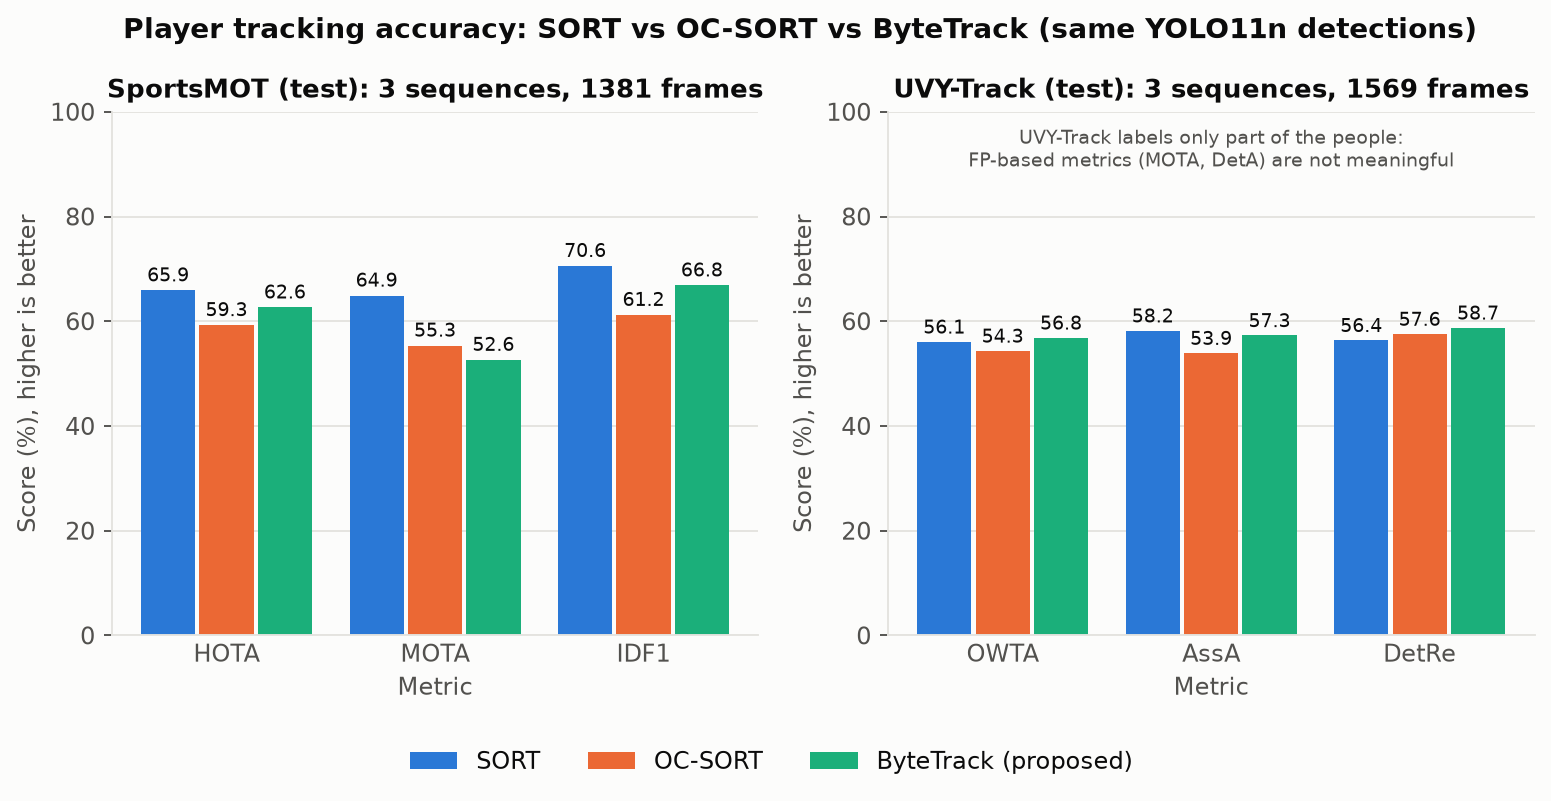
\includegraphics[width=0.86\textwidth]{fig_tracking_accuracy.png}
\caption{Tracking accuracy with tuned parameters. Left: HOTA, MOTA and IDF1 on
SportsMOT. Right: OWTA, AssA and detection recall on UVY-Track.}
\label{fig:tracking}
\end{figure*}

\subsection{Player tracking: baseline comparison on SportsMOT}
Table~\ref{tab:sportsmot} and Fig.~\ref{fig:tracking} report the three trackers
on the SportsMOT test sequences. ByteTrack makes the fewest identity switches
(51, against 60 for SORT and 106 for
OC-SORT) and misses the fewest players (670 false negatives, recall
95.9\%). The tuned SORT, however, has the best HOTA
(65.9 against 62.6), MOTA (64.9) and IDF1
(70.6). The two are close in association (AssA 67.0 and
66.1); the difference is detection accuracy, because ByteTrack
outputs 2{,}131 more false-positive boxes. Its second matching stage
keeps tracks alive on low-confidence boxes, which with a benchmark-trained
detector are occluded players, but with a generic detector are often unannotated
people at the edge of the pitch. OC-SORT is the weakest associator here.

With one shared, untuned setting the three trackers lie within
0.8 HOTA points (lower half of Table~\ref{tab:sportsmot}), and
ByteTrack again has the fewest identity switches (43). The
tuning sequence contains few unannotated people, so a low confidence threshold
looked best for OC-SORT there and then cost it on the test sequences
(Fig.~\ref{fig:tuning}); tuning on a single sequence is a limitation of this
study.

\begin{figure}[!htb]
\centering
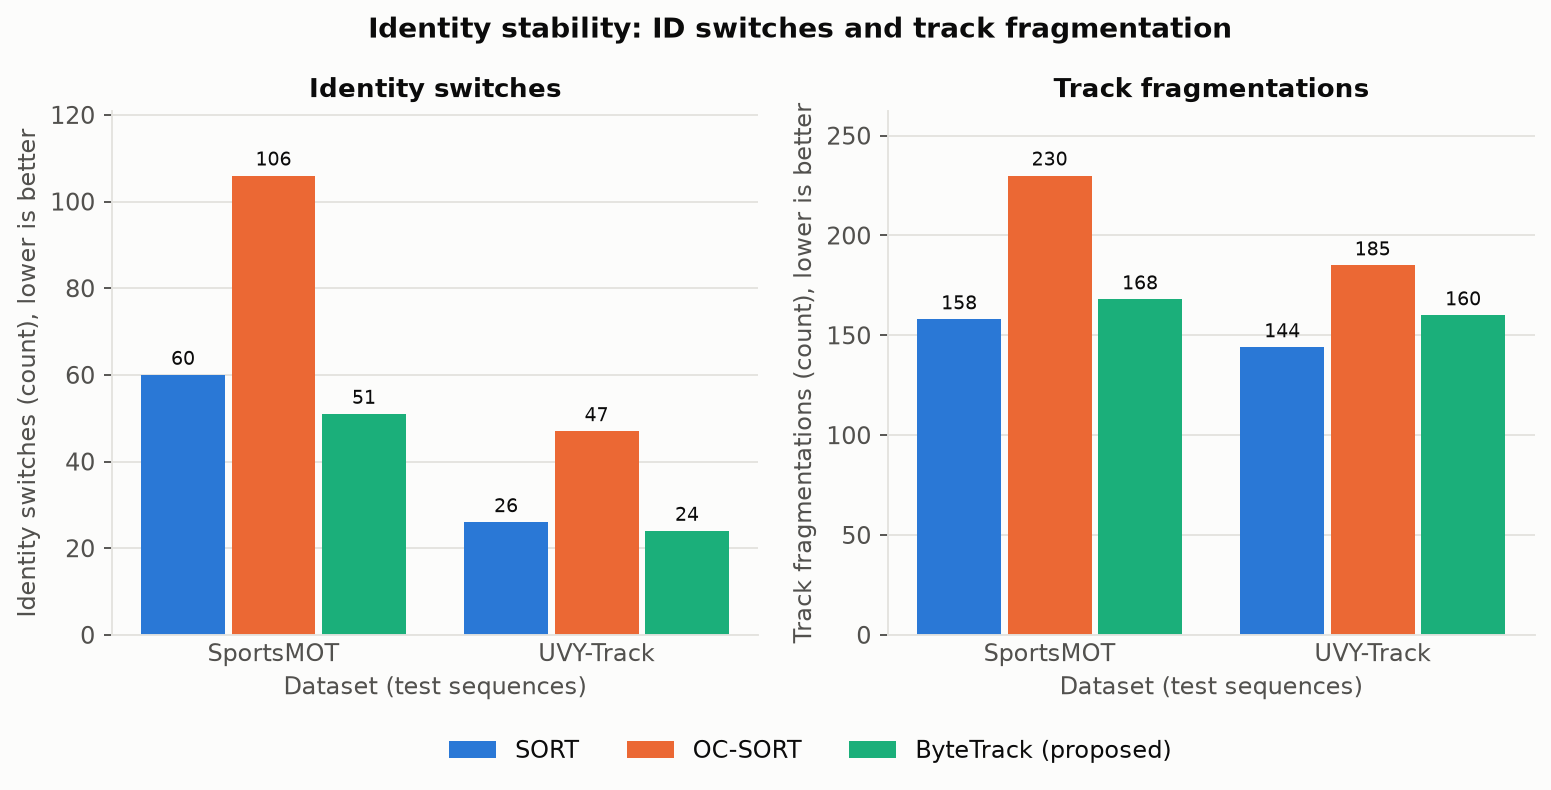
\includegraphics[width=\columnwidth]{fig_idsw_frag.png}
\caption{Identity switches and fragmentations on the test sequences (lower is
better).}
\label{fig:idsw}
\end{figure}

\begin{figure}[!htb]
\centering
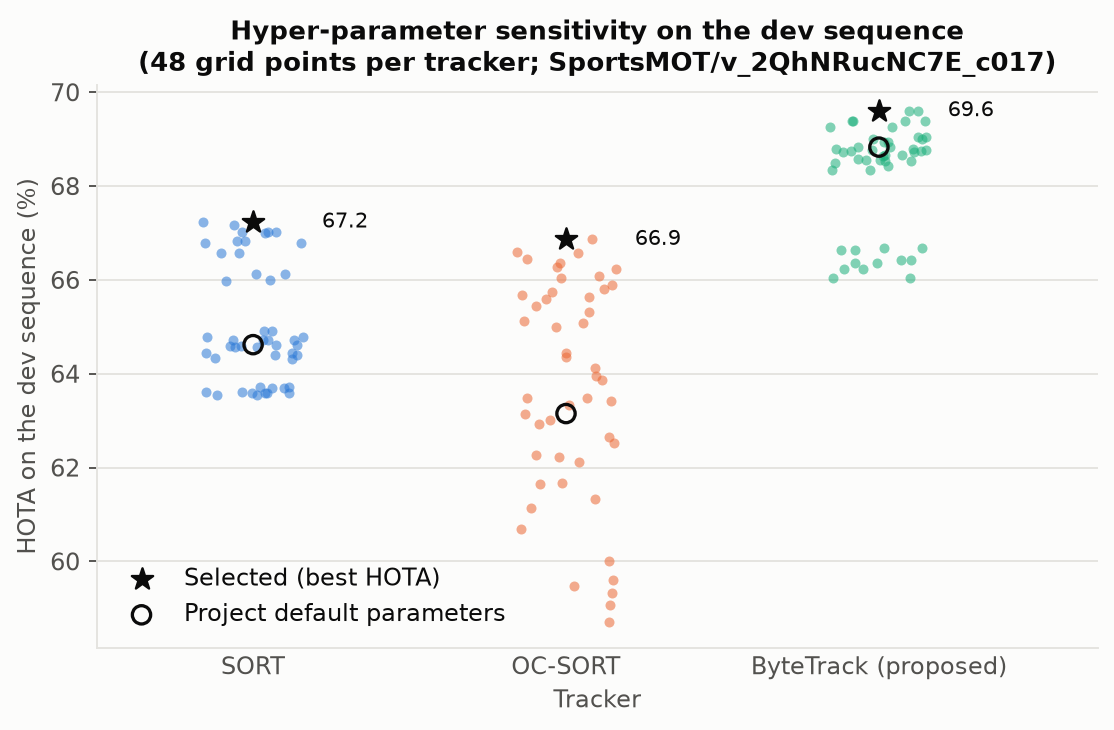
\includegraphics[width=0.9\columnwidth]{fig_tuning.png}
\caption{HOTA on the tuning sequence for the 48 settings of each tracker. Star:
selected setting; circle: shared default.}
\label{fig:tuning}
\end{figure}

\begin{figure*}[!t]
\centering
\includegraphics[width=\textwidth]{fig_sota.png}
\caption{Left: HOTA of published SportsMOT results and of our trackers. Right:
detection against association accuracy with iso-HOTA curves; our trackers sit at
the same association level as the best published methods but far lower in
detection.}
\label{fig:sota}
\end{figure*}

\subsection{Player tracking on UVY-Track}
On UVY-Track (Table~\ref{tab:uvy}) the trackers are close. ByteTrack has the best
OWTA (56.8), the highest detection recall (58.7) and
the fewest identity switches (24), whereas OC-SORT has nearly twice
as many (47). Fig.~\ref{fig:idsw} summarises identity stability
on both datasets.

\begin{table}[!htb]
\caption{Player tracking on UVY-Track (tuned parameters); only metrics that do
not count false positives}
\label{tab:uvy}
\centering
\footnotesize
\begin{adjustbox}{max width=\columnwidth}
\begin{tabular}{@{}lrrrrrrr@{}}
\toprule
Tracker & OWTA & DetRe & AssA & IDSW & Frag & MT & FN \\
\midrule
SORT & 56.1 & 56.4 & \textbf{58.2} & 26 & \textbf{144} & \textbf{16} & 2{,}524 \\
OC-SORT & 54.3 & 57.6 & 53.9 & 47 & 185 & \textbf{16} & 2{,}363 \\
ByteTrack (proposed) & \textbf{56.8} & \textbf{58.7} & 57.3 & \textbf{24} & 160 & \textbf{16} & \textbf{2{,}232} \\
\bottomrule
\end{tabular}
\end{adjustbox}
\end{table}

\begin{table*}[!t]
\caption{Ball results on identical candidates. Coverage: share of scored frames
with an output. Frames: detected, predicted, no output. Segments: number and
mean length of correctly tracked segments}
\label{tab:ball}
\centering
\footnotesize
\begin{adjustbox}{max width=\textwidth}
\begin{tabular}{@{}llrrrrrrrrrrrrr@{}}
\toprule
 & & \multicolumn{3}{c}{Distance criterion (\%)} & \multicolumn{3}{c}{IoU $\geq 0.5$ (\%)} & AP@0.5 & Cover. & \multicolumn{3}{c}{Frames} & \multicolumn{2}{c}{Segments} \\
\cmidrule(lr){3-5}\cmidrule(lr){6-8}\cmidrule(lr){11-13}\cmidrule(lr){14-15}
Data & Method & Prec. & Rec. & F1 & Prec. & Rec. & F1 & (\%) & (\%) & Det. & Pred. & None & No. & Mean len. \\
\midrule
UVY-Track & Detection only & 64.3 & 48.7 & 55.4 & 27.4 & 20.7 & 23.6 & 17.8 & 75.7 & 782 & 0 & 251 & 88 & 5.7 \\
UVY-Track & Kalman, detected only & 58.5 & 34.4 & 43.3 & 36.1 & 21.2 & 26.7 & -- & 58.8 & 607 & 0 & 426 & 32 & 11.1 \\
UVY-Track & Kalman (YOLO only) & 58.2 & 42.8 & 49.3 & 30.7 & 22.6 & 26.0 & -- & 73.5 & 607 & 152 & 274 & 8 & 55.2 \\
UVY-Track & Kalman + motion (proposed) & 59.0 & 44.1 & 50.5 & 32.0 & 23.9 & 27.4 & -- & 74.8 & 621 & 152 & 260 & 9 & 50.7 \\
\midrule
InFactory & Detection only & 74.5 & 34.4 & 47.1 & 66.9 & 30.9 & 42.3 & 26.0 & 28.1 & 408 & 0 & 1{,}042 & 73 & 4.2 \\
InFactory & Kalman, detected only & 92.5 & 27.8 & 42.8 & 80.1 & 24.1 & 37.0 & -- & 18.3 & 266 & 0 & 1{,}184 & 50 & 4.9 \\
InFactory & Kalman (YOLO only) & 82.5 & 36.9 & 51.0 & 63.5 & 28.4 & 39.2 & -- & 27.2 & 266 & 129 & 1{,}055 & 33 & 9.9 \\
InFactory & Kalman + motion (proposed) & 82.5 & 36.9 & 51.0 & 63.3 & 28.3 & 39.1 & -- & 27.2 & 269 & 126 & 1{,}055 & 33 & 9.9 \\
\midrule
All (13 seq.) & Detection only & 67.8 & 42.1 & 51.9 & 40.9 & 25.4 & 31.3 & 20.5 & 47.9 & 1{,}190 & 0 & 1{,}293 & 161 & 5.0 \\
All (13 seq.) & Kalman, detected only & 68.8 & 31.4 & 43.1 & 49.5 & 22.5 & 31.0 & -- & 35.2 & 873 & 0 & 1{,}610 & 82 & 7.3 \\
All (13 seq.) & Kalman (YOLO only) & 66.6 & 40.1 & 50.0 & 41.9 & 25.2 & 31.5 & -- & 46.5 & 873 & 281 & 1{,}329 & 41 & 18.7 \\
All (13 seq.) & Kalman + motion (proposed) & 67.0 & 40.8 & 50.7 & 42.6 & 25.9 & 32.2 & -- & 47.0 & 890 & 278 & 1{,}315 & 42 & 18.6 \\
\bottomrule
\end{tabular}
\end{adjustbox}
\end{table*}

\subsection{Comparison with the state of the art}
Table~\ref{tab:sota} lists 16 published results on the SportsMOT test
set, taken from the source papers~\cite{sportsmot,deepeiou,diffmot}, next to our
three trackers. The protocols differ: the published methods train their detector
on SportsMOT and are scored on the full test set, whereas our detector has never
seen SportsMOT and is scored on three football validation sequences. The
comparison places the project in context; it is not a leaderboard entry.

\begin{table}[!htb]
\caption{Published SportsMOT test results~\cite{sportsmot,deepeiou,diffmot}
and ours ($^{*}$: detector trained on train+val)}
\label{tab:sota}
\centering
\footnotesize
\begin{adjustbox}{max width=\columnwidth}
\begin{tabular}{@{}lrrrrr@{}}
\toprule
Method & HOTA & DetA & AssA & MOTA & IDF1 \\
\midrule
FairMOT & 49.3 & 70.2 & 34.7 & 86.4 & 53.5 \\
GTR & 54.5 & 64.8 & 45.9 & 67.9 & 55.8 \\
QDTrack & 60.4 & 77.5 & 47.2 & 90.1 & 62.3 \\
CenterTrack & 62.7 & 82.1 & 48.0 & 90.8 & 60.0 \\
ByteTrack & 62.8 & 77.1 & 51.2 & 94.1 & 69.8 \\
ByteTrack$^{*}$ & 64.1 & 78.5 & 52.3 & 95.9 & 71.4 \\
MixSort-Byte$^{*}$ & 65.7 & 78.8 & 54.8 & 96.2 & 74.1 \\
BoT-SORT & 68.7 & 84.4 & 55.9 & 94.5 & 70.0 \\
TransTrack & 68.9 & 82.7 & 57.5 & 92.6 & 71.5 \\
OC-SORT & 71.9 & 86.4 & 59.8 & 94.5 & 72.2 \\
DiffMOT & 72.1 & 86.0 & 60.5 & 94.5 & 72.8 \\
OC-SORT$^{*}$ & 73.7 & 88.5 & 61.5 & 96.5 & 74.0 \\
Deep-EIoU & 74.1 & 87.2 & 63.1 & 95.1 & 75.0 \\
MixSort-OC$^{*}$ & 74.1 & 88.5 & 62.0 & 96.5 & 74.4 \\
DiffMOT$^{*}$ & 76.2 & 89.3 & 65.1 & 97.1 & 76.1 \\
Deep-EIoU$^{*}$ & 77.2 & 88.2 & 67.7 & 96.3 & 79.8 \\
\midrule
\textit{Ours: YOLO11n + SORT} & 65.9 & 64.8 & 67.0 & 64.9 & 70.6 \\
\textit{Ours: YOLO11n + OC-SORT} & 59.3 & 60.6 & 58.0 & 55.3 & 61.2 \\
\textit{Ours: YOLO11n + ByteTrack (proposed)} & 62.6 & 59.4 & 66.1 & 52.6 & 66.8 \\
\bottomrule
\end{tabular}
\end{adjustbox}
\end{table}

\begin{figure*}[!t]
\centering
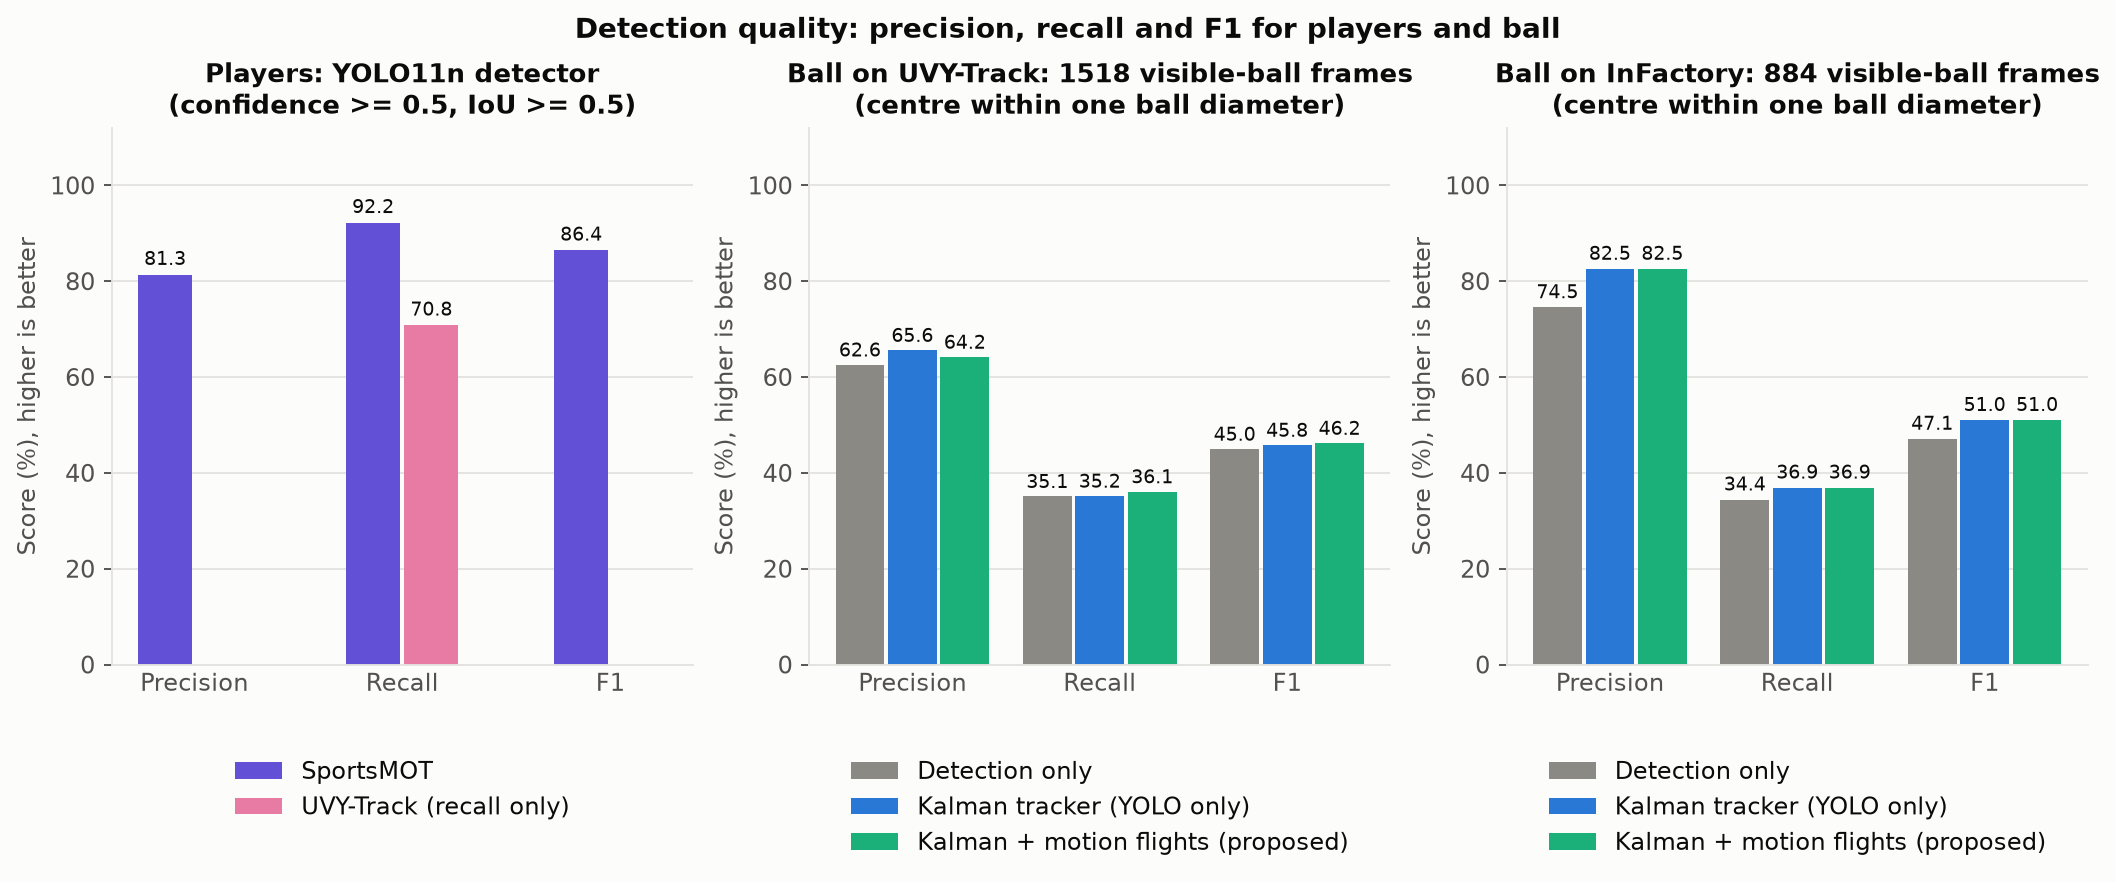
\includegraphics[width=\textwidth]{fig_detection_prf.png}
\caption{Precision, recall and F1 for player detection (left) and for the ball
on UVY-Track and InFactory (distance criterion).}
\label{fig:prf}
\end{figure*}

Fig.~\ref{fig:sota} shows where the gap lies. The best published tracker,
Deep-EIoU (train+val), reaches HOTA 77.2 with DetA 88.2
and AssA 67.7. Our ByteTrack trails it by only 1.6 points in
AssA but by 28.8 points in DetA. Our ByteTrack and the published
ByteTrack reach almost the same HOTA (62.6 and 62.8) for
opposite reasons: theirs detects better (DetA 77.1), ours associates
better on three football clips (AssA 66.1 against
51.2), which should not be read as a better tracker. The tracker
ranking also depends on the detector: with a benchmark-trained detector OC-SORT
is far ahead of ByteTrack (71.9 against 62.8), with ours
it is behind. Both observations point to the detector, not the association
algorithm, as the component to improve.

\subsection{Ball detection and tracking}
Table~\ref{tab:ball} and Fig.~\ref{fig:prf} compare four ball outputs on the same
candidates: the most confident detection per frame (detection only), the
detections accepted by the Kalman tracker, the full Kalman tracker, and the
Kalman tracker with motion flights.

The detector limits everything that follows: the COCO \emph{sports ball} class
finds the ball in well under half of the frames in which it is visible, and the
average precision of all its candidates is only 20.5\%. On the held-out
InFactory clips the tracker helps: F1 rises from 47.1 to
51.0 and precision from 74.5 to 82.5. On
UVY-Track detection alone is better (F1 55.4 against
50.5), so over all 13 sequences detection alone has the
slightly higher F1 (51.9 against 50.7). The clearest gain
is continuity: 161 short, correctly tracked pieces merge into
42 longer ones. Detections accepted by the tracker are more
precise than predicted positions (69.4\% against 59.0\%), which is
why predictions are reported separately (Table~\ref{tab:ballpred}).
Fig.~\ref{fig:ballstatus} shows the share of detected, predicted and missing
ball outputs for each sequence.

\begin{table}[!htb]
\caption{Kalman tracker with motion flights: precision of detected and of
predicted ball positions (distance criterion)}
\label{tab:ballpred}
\centering
\footnotesize
\begin{adjustbox}{max width=\columnwidth}
\begin{tabular}{@{}lrrrr@{}}
\toprule
 & \multicolumn{2}{c}{Detected} & \multicolumn{2}{c}{Predicted} \\
\cmidrule(lr){2-3}\cmidrule(lr){4-5}
Data & Frames & Prec. (\%) & Frames & Prec. (\%) \\
\midrule
UVY-Track & 621 & 59.4 & 152 & 57.2 \\
InFactory & 269 & 92.6 & 126 & 61.1 \\
All & 890 & 69.4 & 278 & 59.0 \\
\bottomrule
\end{tabular}
\end{adjustbox}
\end{table}

Motion flights change the output on 1 of the 13 ball
sequences. On the free-kick clip \texttt{soccer\_V04} they follow the shot into
the net and raise recall from 91.1\% to 99.4\% at
100.0\% precision (Fig.~\ref{fig:balltraj}). Because the flight rules
were developed on UVY-Track clips, this is not held-out evidence, and on the
held-out InFactory clips the flights left the distance-criterion results
unchanged.

\begin{figure}[!htb]
\centering
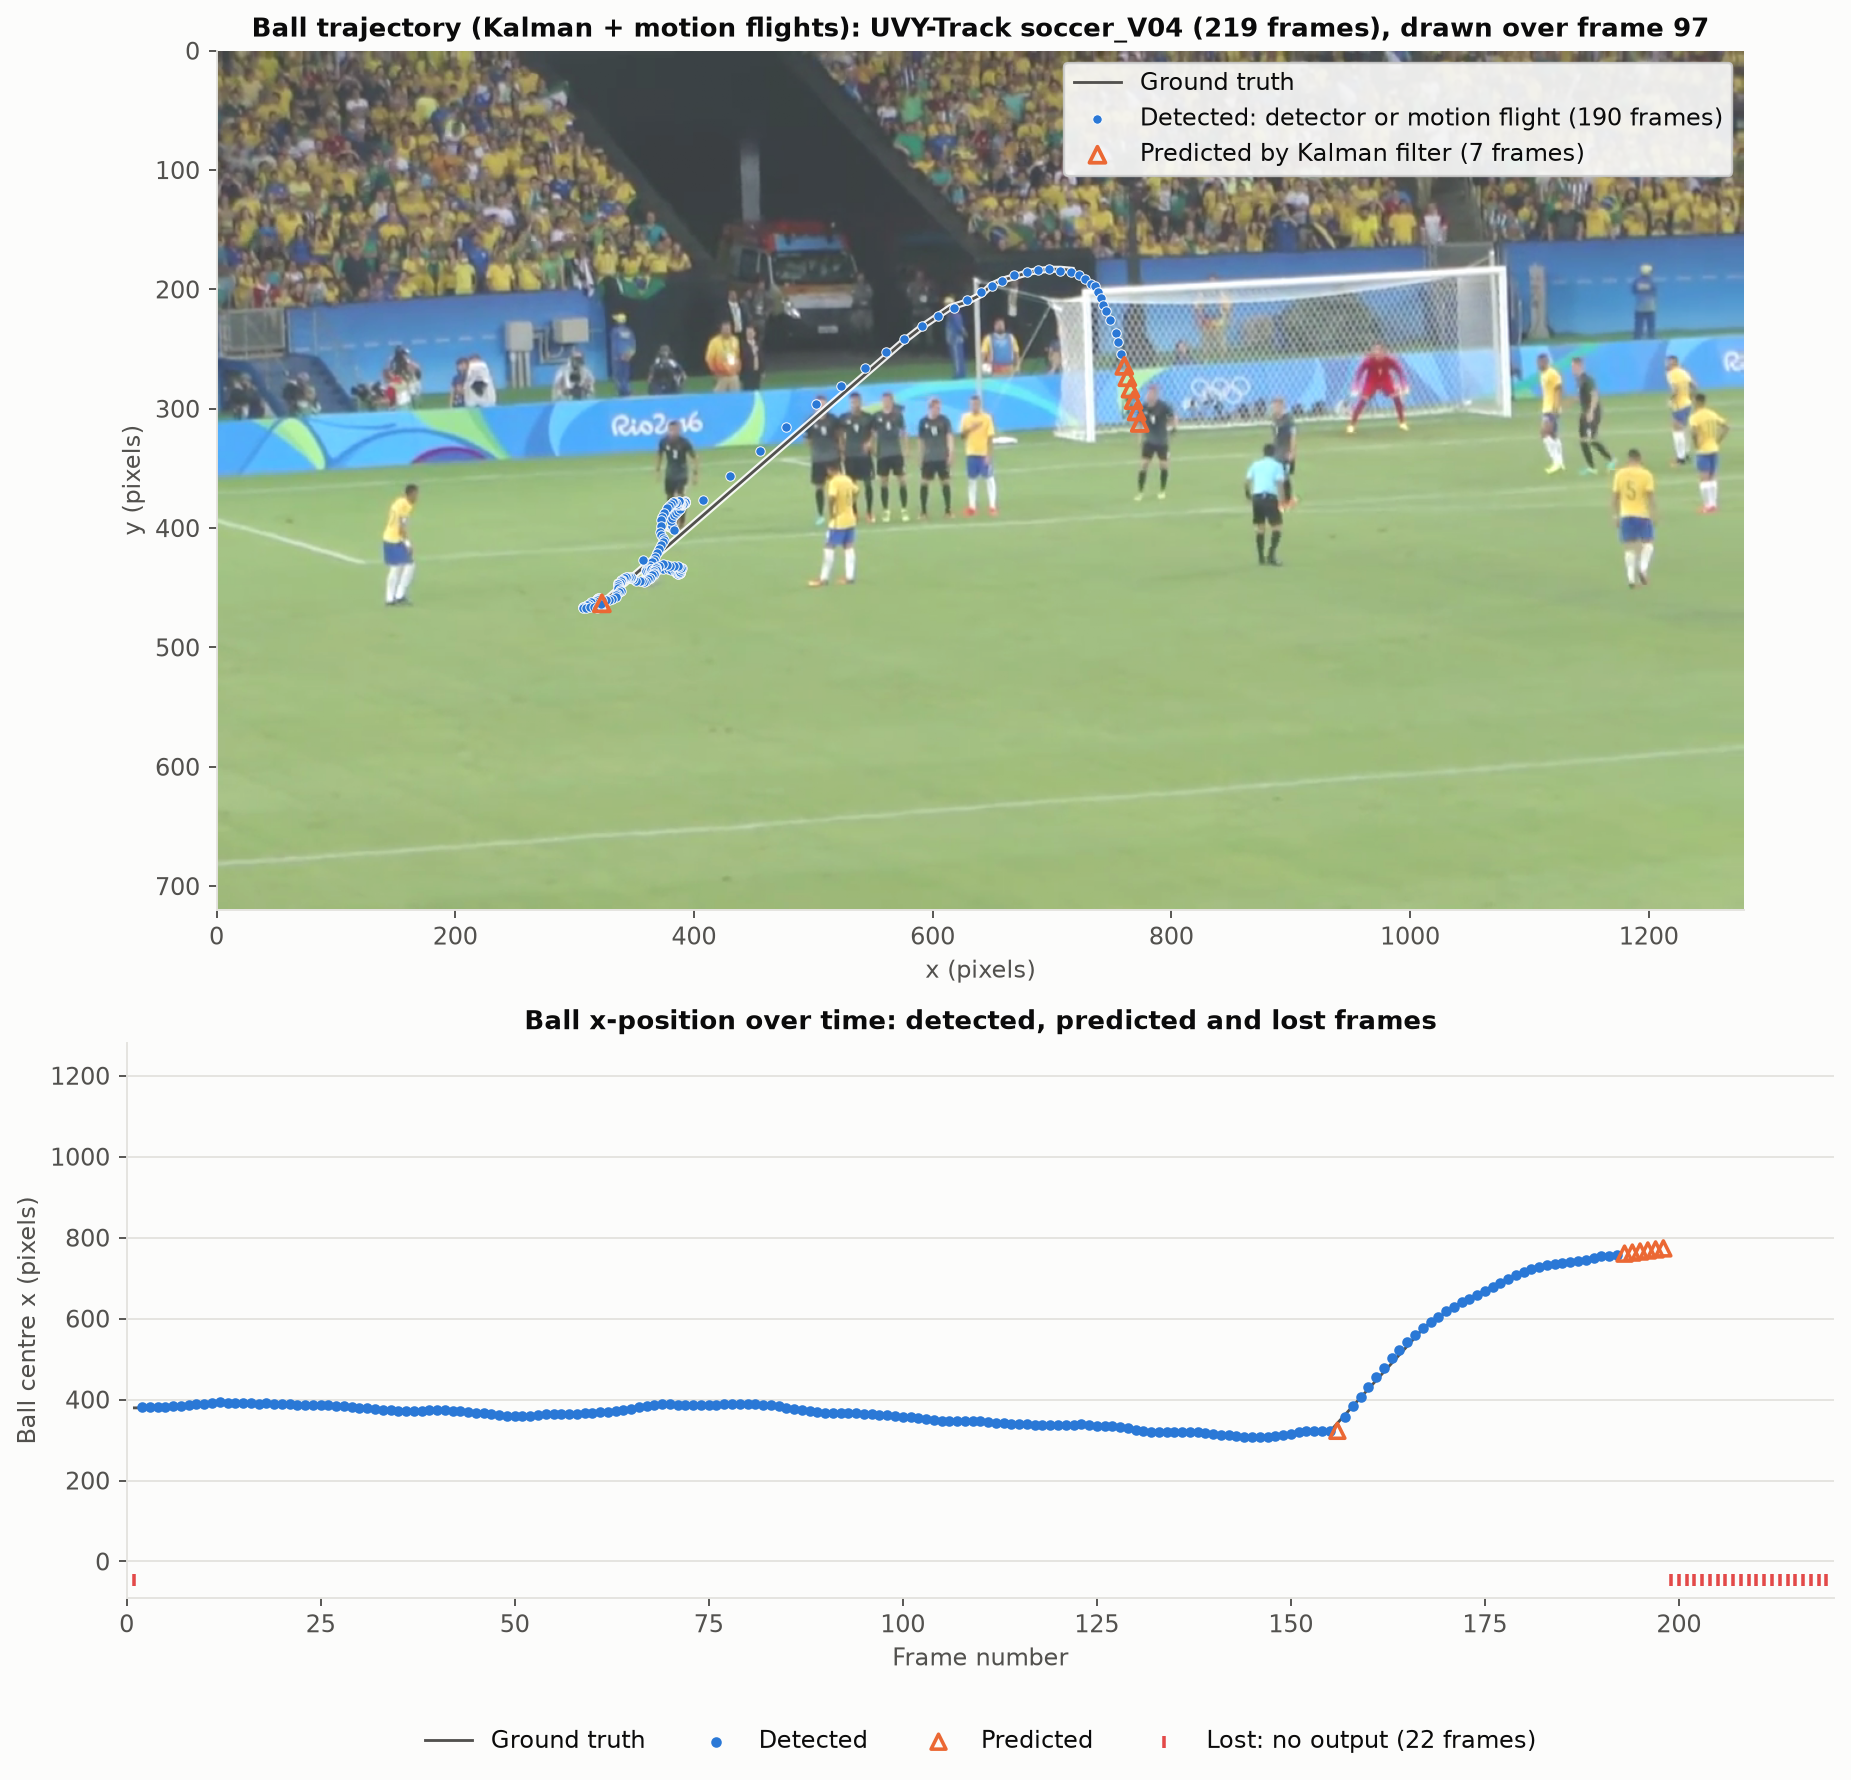
\includegraphics[width=\columnwidth]{fig_ball_trajectory.png}
\caption{Ball trajectory on \texttt{soccer\_V04} with the ground truth. Dots:
detected or flight positions; triangles: Kalman predictions; marks on the time
axis: frames without output.}
\label{fig:balltraj}
\end{figure}

\begin{figure}[!htb]
\centering
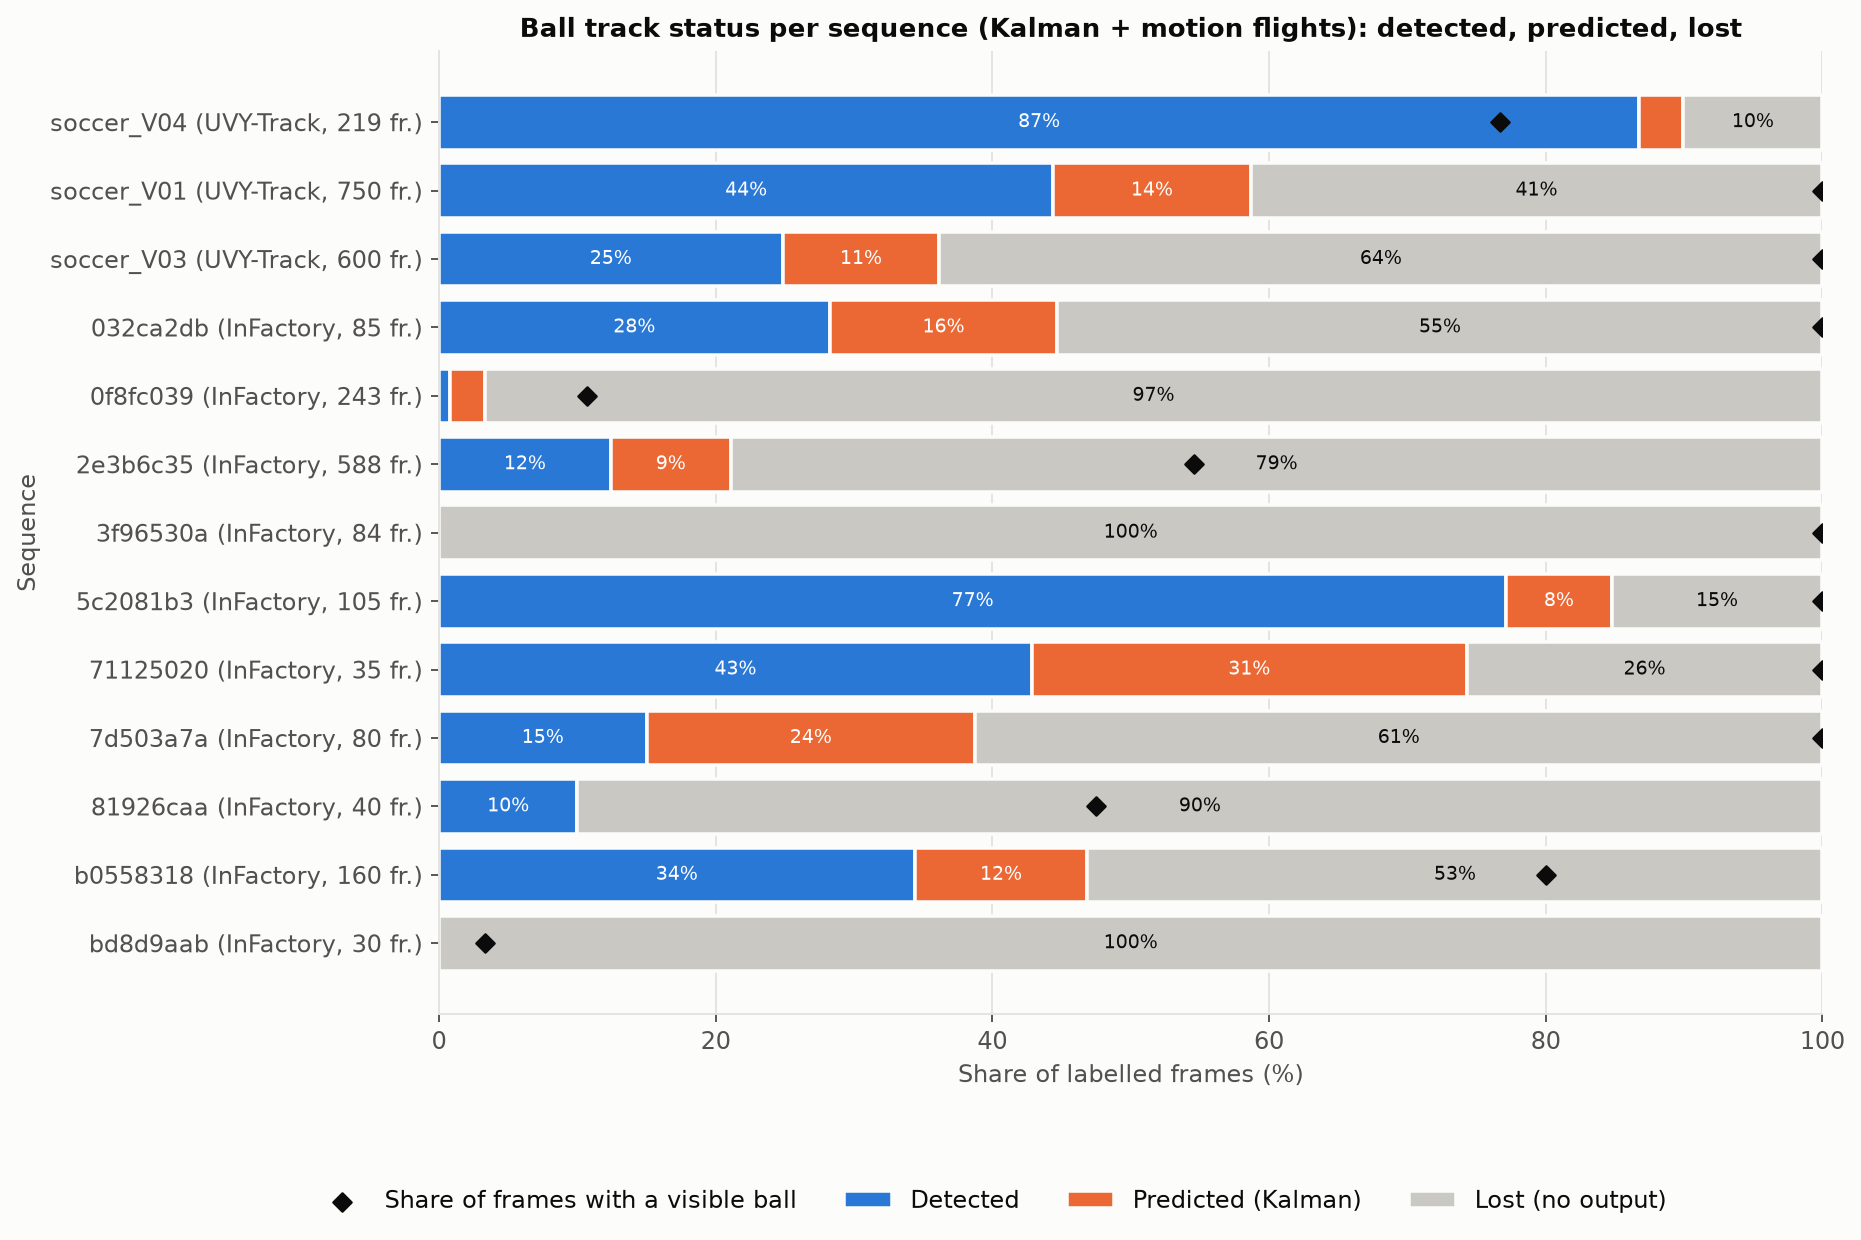
\includegraphics[width=\columnwidth]{fig_ball_status.png}
\caption{Share of detected, predicted and missing ball outputs per sequence.
Diamonds: share of frames with a visible ball.}
\label{fig:ballstatus}
\end{figure}

\begin{figure*}[!t]
\centering
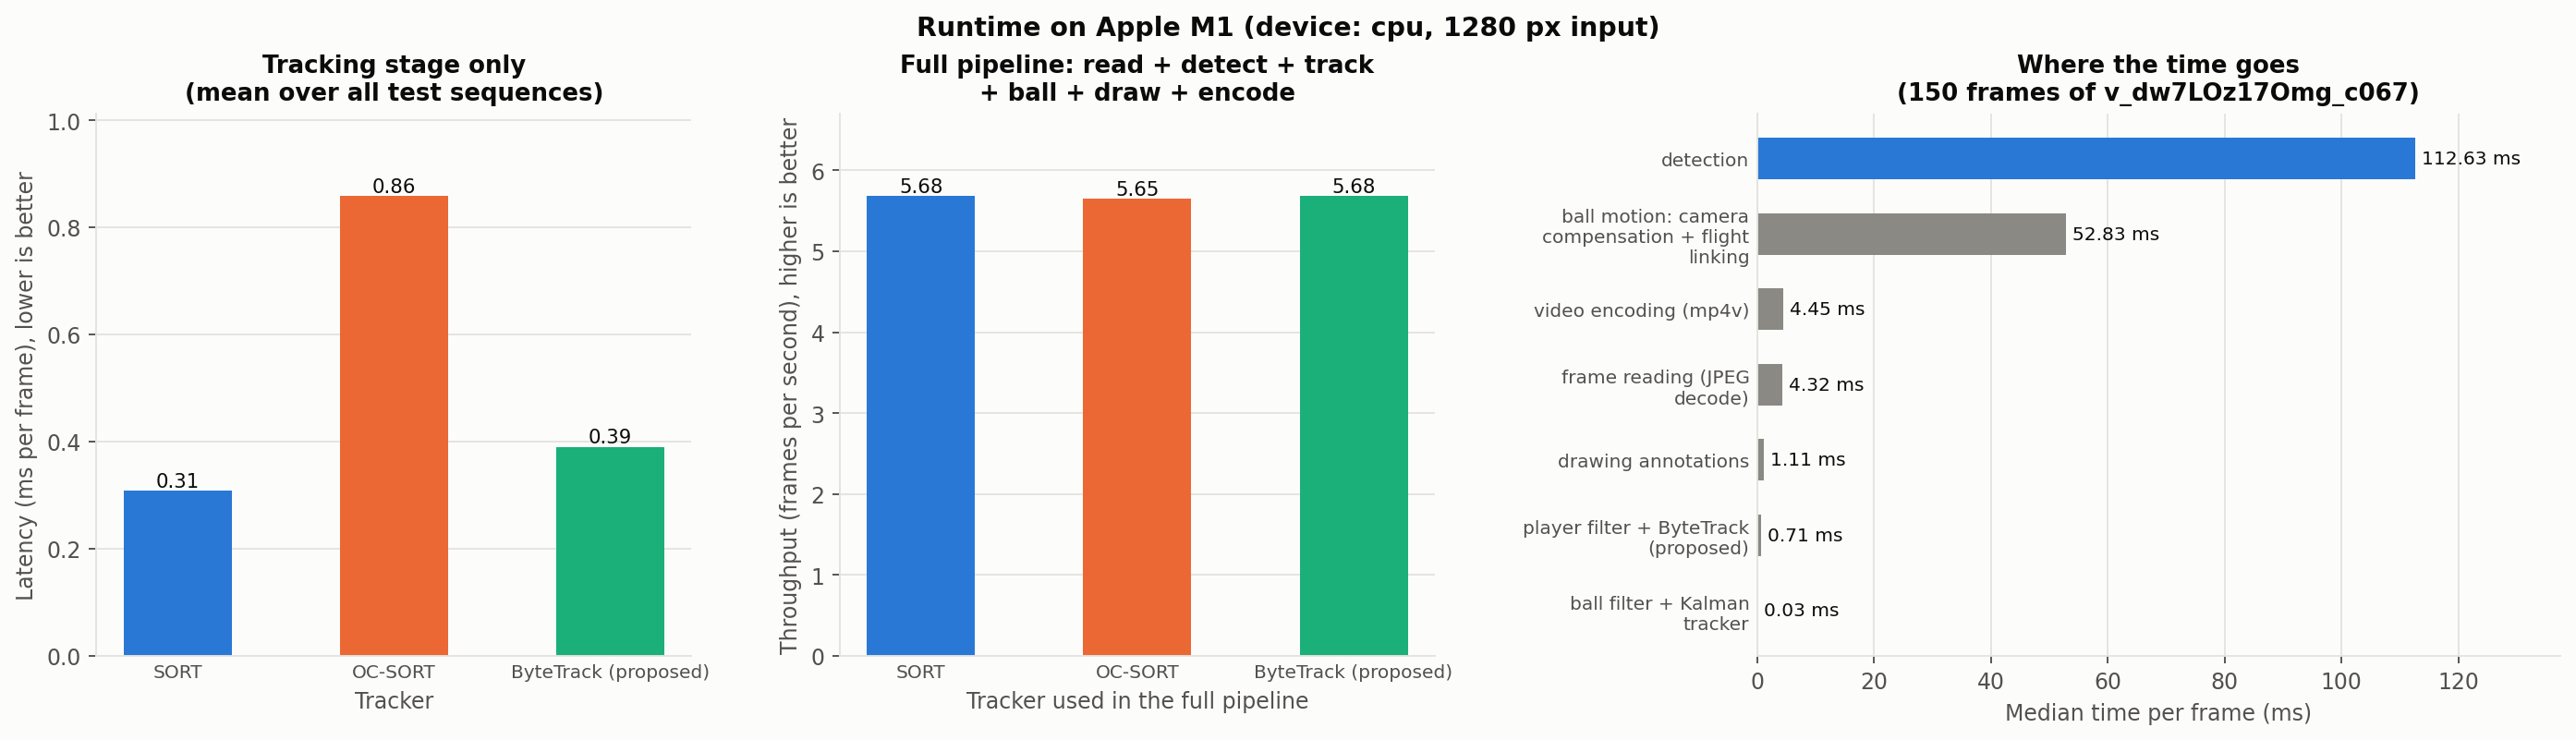
\includegraphics[width=\textwidth]{fig_runtime.png}
\caption{Runtime: tracking stage alone (left), full pipeline throughput (centre)
and time per stage (right).}
\label{fig:runtime}
\end{figure*}

\subsection{Detector comparison}
YOLOv8n and YOLO11n were compared with identical settings on the first 200
frames of one SportsMOT sequence and on two InFactory clips
(Table~\ref{tab:models}); speed was measured by alternating the two models frame
by frame. YOLO11n detects players more precisely and is faster; for the ball the
two are practically equal. The sample is small, but it supports the choice of
YOLO11n.

\begin{table}[!htb]
\caption{YOLOv8n versus YOLO11n on the same frames}
\label{tab:models}
\centering
\footnotesize
\begin{adjustbox}{max width=\columnwidth}
\begin{tabular}{@{}llrrrrrr@{}}
\toprule
Model & Target & Frames & Prec. & Rec. & F1 & AP@0.5 & ms/fr. \\
\midrule
YOLOv8n & player & 200 & 60.9 & 87.1 & 71.7 & 71.7 & 112 \\
YOLOv8n & ball & 265 & 83.0 & 67.0 & 74.1 & 51.0 & 112 \\
YOLO11n & player & 200 & 74.5 & 89.2 & 81.2 & 79.0 & 106 \\
YOLO11n & ball & 265 & 88.8 & 64.8 & 74.9 & 51.2 & 106 \\
\bottomrule
\end{tabular}
\end{adjustbox}
\end{table}

\subsection{Runtime}
The full pipeline processes 5.7 frames per second on the Apple M1
(Table~\ref{tab:runtime}, Fig.~\ref{fig:runtime}). The detector takes
64\% of the time (113~ms per frame) and the ball motion
stage 30\% (53~ms), while ByteTrack needs only
0.71~ms. The choice of player tracker therefore hardly affects speed,
and the system is an offline analysis tool on this hardware. On battery power
the laptop processor throttles and throughput drops markedly.

\begin{table}[!htb]
\caption{Median processing time per frame}
\label{tab:runtime}
\centering
\footnotesize
\begin{adjustbox}{max width=\columnwidth}
\begin{tabular}{@{}lrr@{}}
\toprule
Stage & Time (ms) & Share (\%) \\
\midrule
Detection & 112.63 & 64.0 \\
Ball motion: camera compensation + flight linking & 52.83 & 30.0 \\
Video encoding & 4.45 & 2.5 \\
Frame reading & 4.32 & 2.5 \\
Drawing annotations & 1.11 & 0.6 \\
Player filter + ByteTrack & 0.71 & 0.4 \\
Ball filter + Kalman tracker & 0.03 & 0.0 \\
\midrule
\textbf{Total (proposed pipeline)} & \textbf{176.1} & 100.0 \\
\midrule
Player filter + SORT (baseline) & 0.61 & -- \\
Player filter + OC-SORT (baseline) & 1.59 & -- \\
\bottomrule
\end{tabular}
\end{adjustbox}
\end{table}

\subsection{Qualitative results}
Fig.~\ref{fig:demo} shows a frame of the annotated output for the UVY-Track
clip \texttt{soccer\_V04}. Figs.~\ref{fig:trajectories} and~\ref{fig:heatmap}
show player trajectories and a position heatmap for a SportsMOT sequence, both
in image coordinates.

\begin{figure}[!htb]
\centering
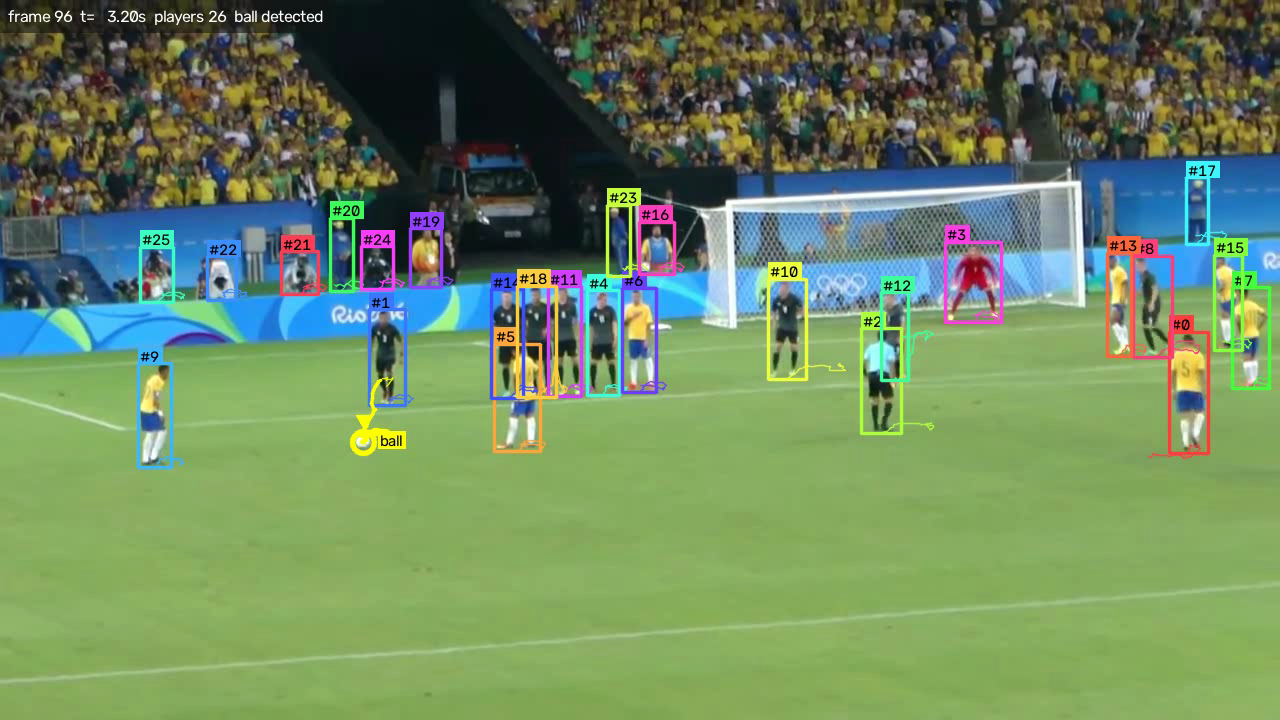
\includegraphics[width=\columnwidth]{fig_demo_screenshot.png}
\caption{Annotated output: player identities and trails, the ball and its recent
path, and a status line.}
\label{fig:demo}
\end{figure}

\begin{figure}[!htb]
\centering
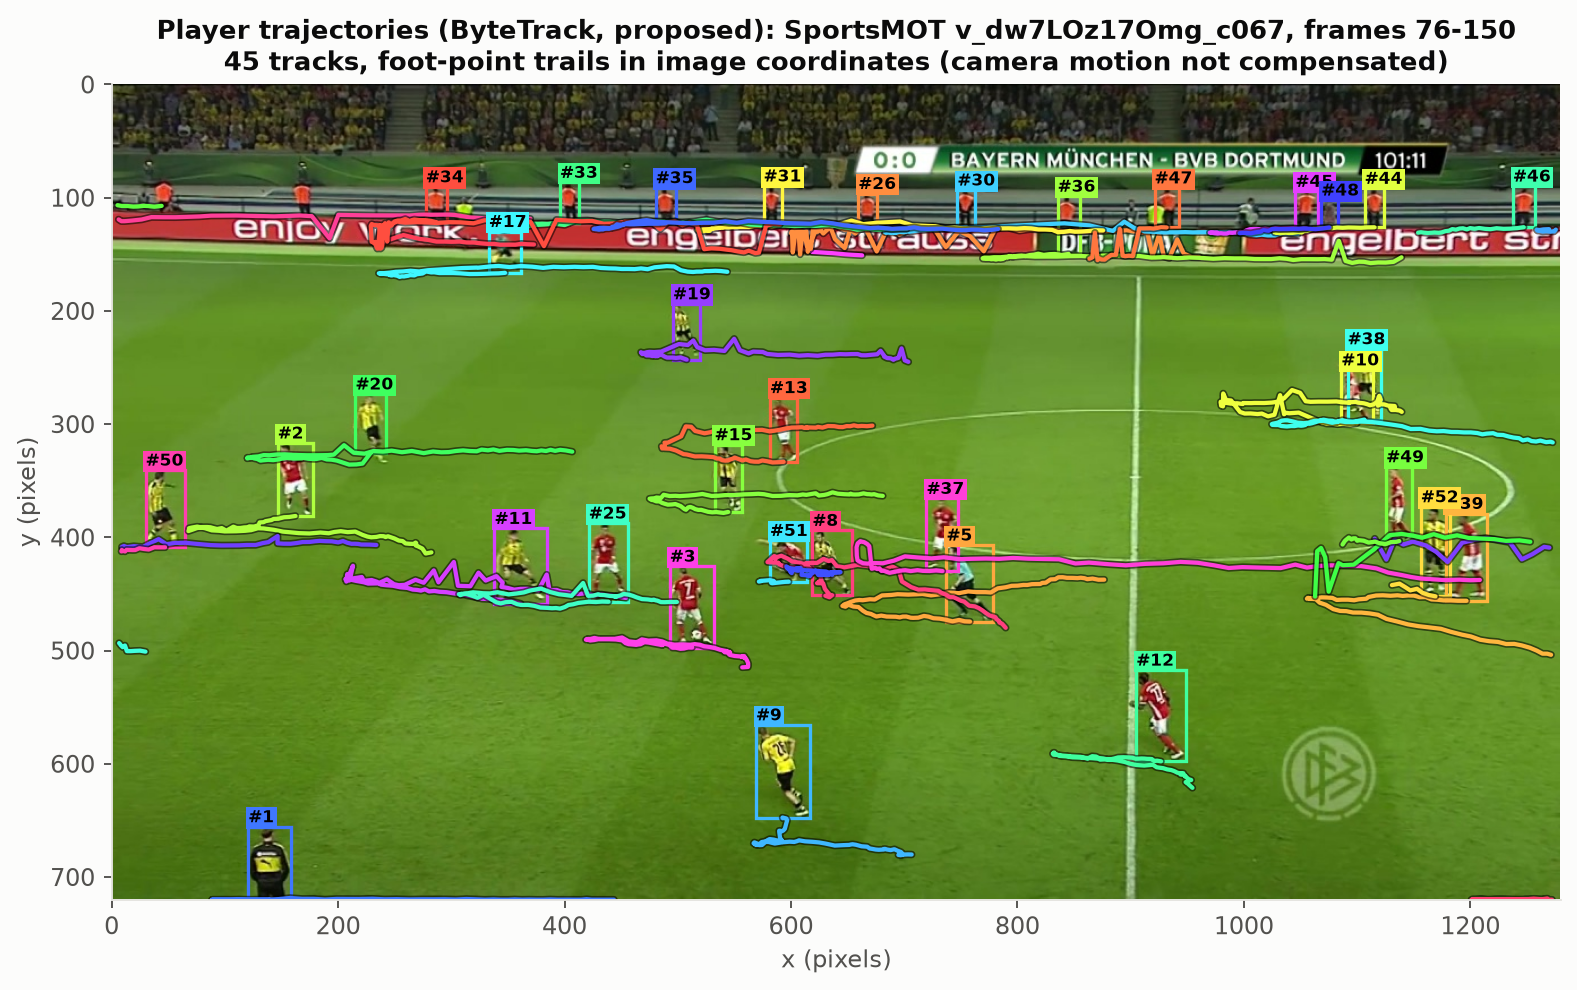
\includegraphics[width=\columnwidth]{fig_player_trajectories.png}
\caption{Player trajectories from ByteTrack over 75 frames of a SportsMOT test
sequence. Tracks along the top are perimeter staff, detected and tracked but not
annotated in the benchmark.}
\label{fig:trajectories}
\end{figure}

\begin{figure}[!htb]
\centering
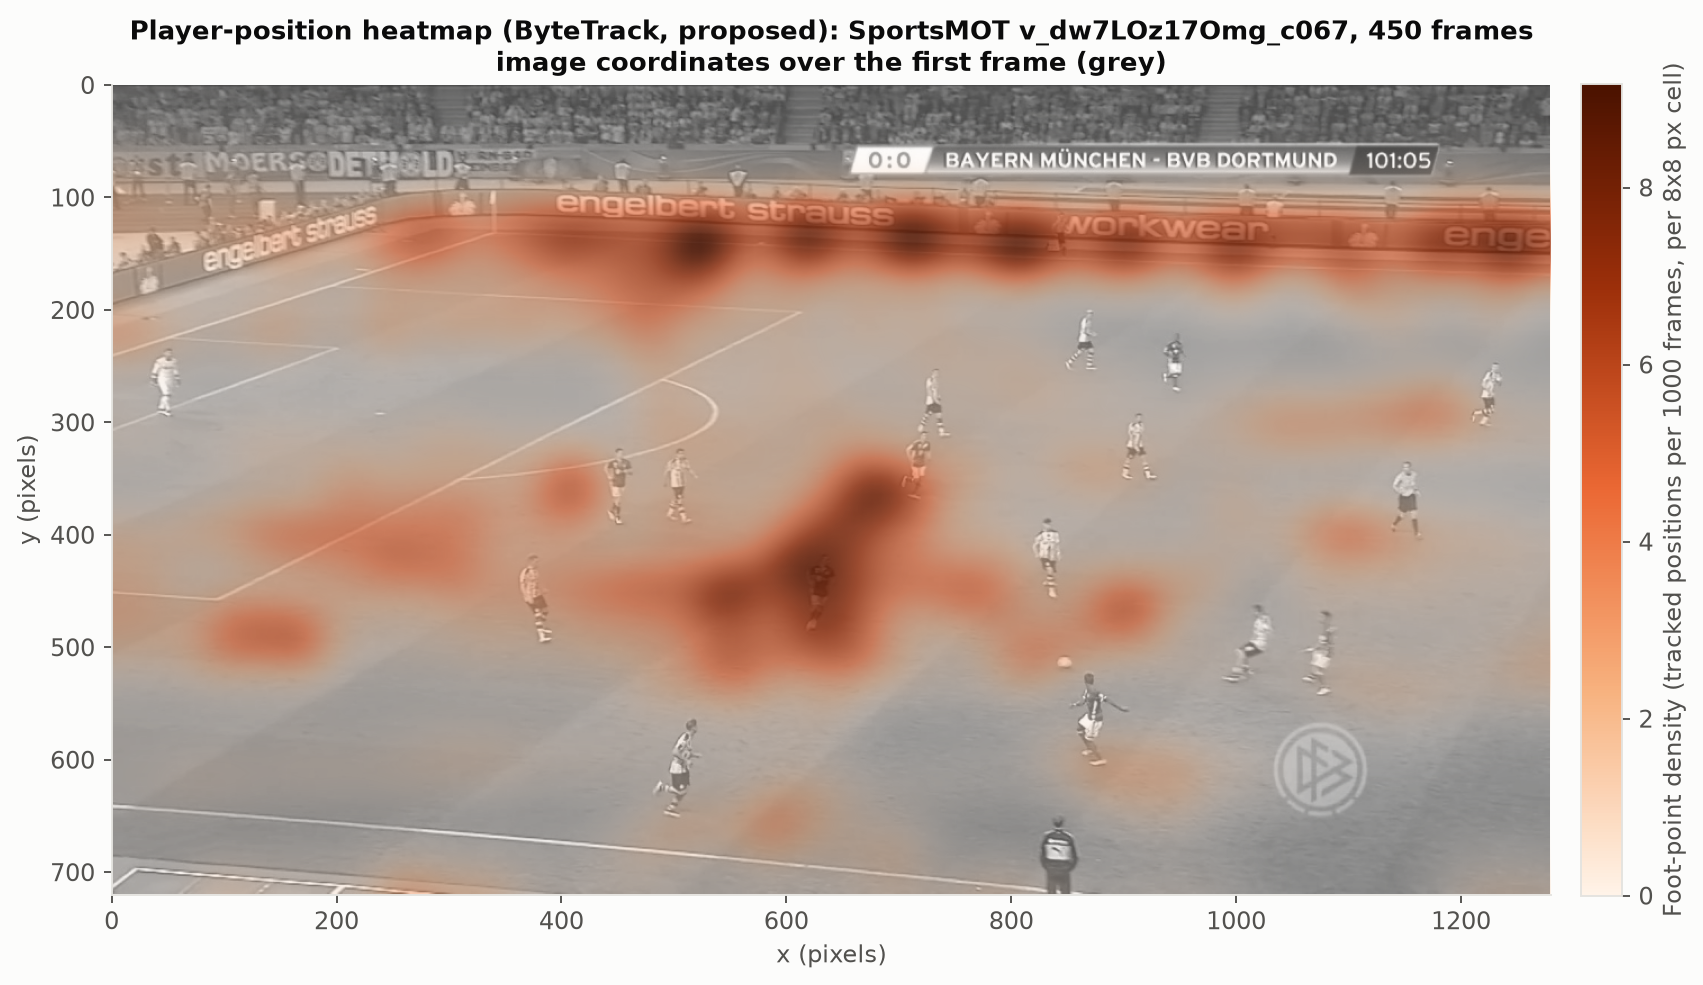
\includegraphics[width=\columnwidth]{fig_player_heatmap.png}
\caption{Player-position heatmap for the same sequence.}
\label{fig:heatmap}
\end{figure}

% Print every Results figure and table before the Discussion starts.
\FloatBarrier

% =============================================================================
\section{Discussion and Limitations}
% =============================================================================
The experiments separate the contribution of the tracker from that of the
detector, and the detector dominates. Its generic \emph{person} class responds
to everybody in view, so the tracker that keeps the most tracks alive is also
penalised the most for false positives; a soccer-trained detector would change
both the absolute numbers and possibly the ranking, as the published results
suggest. The study has further limits. The evaluation covers six tracking test
sequences and 13 ball sequences with a single tuning sequence, and
reports no confidence intervals. No single dataset evaluates the whole system,
because each lacks a different kind of label. A constant-velocity model cannot
follow a ball whose direction changes during a gap, and the ball tracker was not
tuned on separate data. The system has no camera-motion compensation for
players, no re-identification across camera cuts and no team assignment, and it
runs at a few frames per second on a CPU.

% =============================================================================
\section{Individual Contributions}
% =============================================================================
Table~\ref{tab:contrib} lists who owned each part of the work; the full
component list with the supporting commits is kept in the project repository.

\begin{table}[!htb]
\caption{Individual contributions}
\label{tab:contrib}
\centering
\footnotesize
\begin{tabular}{@{}>{\raggedright\arraybackslash}p{1.45cm}>{\raggedright\arraybackslash}p{4.15cm}>{\raggedright\arraybackslash}p{2.25cm}@{}}
\toprule
Member & Main responsibilities & Answers for (viva) \\
\midrule
Pulapa Yaswanth Kumar & Core application (video input and output, YOLO detection, filters, ByteTrack player tracking, the first Kalman ball tracker, visualisation, CSV and JSON export, command-line interface); baseline trackers and the fair comparison protocol; dataset loaders; evaluation framework; experiment runner, plots and database; automated tests; first full experiment run & ByteTrack, SORT and OC-SORT; Kalman filter; metrics; datasets \\
Ravva Siddhartha & Motion flights for the ball in flight (camera-motion compensation, frame differencing, flight linking); hardening of the Kalman ball tracker; integration of motion flights into the experiments; final regenerated results and result videos; IEEE paper (related work, references) & Motion stage and flight rules; final results; ball tracking changes \\
\bottomrule
\end{tabular}
\end{table}


% =============================================================================
\section{Conclusion and Future Work}
% =============================================================================
We built, tested and evaluated a player-and-ball tracking system for soccer
under a reproducible protocol on three public datasets. With identical
detections, ByteTrack produced the most stable player identities and the best
result on the partially labelled UVY-Track data, while a tuned SORT reached the
highest HOTA on SportsMOT and OC-SORT trailed in association. Placed against
published SportsMOT results, our association accuracy is close to the state of
the art and the remaining gap is in detection. The Kalman ball tracker made the
ball track far more continuous and improved F1 on held-out data, but not on
every dataset, and its predicted positions are kept apart from detections
throughout. The most valuable next step is therefore a detector trained on
soccer data, with separate classes for players, officials and the ball.
Further steps are tiled high-resolution inference for the ball, a motion model
that can handle direction changes, camera-motion compensation and
re-identification for players, team assignment, and an evaluation on the full
benchmark splits.

% =============================================================================
\begin{thebibliography}{00}
\bibitem{sort} A. Bewley, Z. Ge, L. Ott, F. Ramos, and B. Upcroft, ``Simple online and realtime tracking,'' in \emph{Proc. IEEE Int. Conf. Image Process. (ICIP)}, 2016, pp. 3464--3468.
\bibitem{bytetrack} Y. Zhang, P. Sun, Y. Jiang, D. Yu, F. Weng, Z. Yuan, P. Luo, W. Liu, and X. Wang, ``ByteTrack: Multi-object tracking by associating every detection box,'' in \emph{Proc. Eur. Conf. Comput. Vis. (ECCV)}, 2022.
\bibitem{ocsort} J. Cao, J. Pang, X. Weng, R. Khirodkar, and K. Kitani, ``Observation-centric SORT: Rethinking SORT for robust multi-object tracking,'' in \emph{Proc. IEEE/CVF Conf. Comput. Vis. Pattern Recognit. (CVPR)}, 2023.
\bibitem{yolo11} G. Jocher and J. Qiu, ``Ultralytics YOLO11,'' software, 2024. [Online]. Available: \url{https://github.com/ultralytics/ultralytics}
\bibitem{coco} T.-Y. Lin, M. Maire, S. Belongie, J. Hays, P. Perona, D. Ramanan, P. Doll\'ar, and C. L. Zitnick, ``Microsoft COCO: Common objects in context,'' in \emph{Proc. Eur. Conf. Comput. Vis. (ECCV)}, 2014, pp. 740--755.
\bibitem{sportsmot} Y. Cui, C. Zeng, X. Zhao, Y. Yang, G. Wu, and L. Wang, ``SportsMOT: A large multi-object tracking dataset in multiple sports scenes,'' in \emph{Proc. IEEE/CVF Int. Conf. Comput. Vis. (ICCV)}, 2023.
\bibitem{deepeiou} H.-W. Huang, C.-Y. Yang, J. Sun, P.-K. Kim, K.-J. Kim, K. Lee, C.-I. Huang, and J.-N. Hwang, ``Iterative scale-up ExpansionIoU and deep features association for multi-object tracking in sports,'' arXiv:2306.13074, 2023.
\bibitem{diffmot} W. Lv, Y. Huang, N. Zhang, R.-S. Lin, M. Han, and D. Zeng, ``DiffMOT: A real-time diffusion-based multiple object tracker with non-linear prediction,'' arXiv:2403.02075, 2024.
\bibitem{uvy} E. Alencar and R. de Freitas, ``UVY: A dataset of sport user-generated videos from YouTube for multi-object tracking evaluation,'' Zenodo, 2026. [Online]. Available: \url{https://zenodo.org/records/21303900}
\bibitem{infactory} V. Constantinou, M. Iranmanesh, and J. Kanalakis, ``Soccer ball tracking dataset,'' Infactory, 2026. [Online]. Available: \url{https://huggingface.co/datasets/infactory-ai/ball-tracking}
\bibitem{kalman} R. E. Kalman, ``A new approach to linear filtering and prediction problems,'' \emph{J. Basic Eng.}, vol. 82, no. 1, pp. 35--45, 1960.
\bibitem{hota} J. Luiten, A. O\v{s}ep, P. Dendorfer, P. Torr, A. Geiger, L. Leal-Taix\'e, and B. Leibe, ``HOTA: A higher order metric for evaluating multi-object tracking,'' \emph{Int. J. Comput. Vis.}, vol. 129, 2021.
\bibitem{clear} K. Bernardin and R. Stiefelhagen, ``Evaluating multiple object tracking performance: The CLEAR MOT metrics,'' \emph{EURASIP J. Image Video Process.}, 2008.
\bibitem{idf1} E. Ristani, F. Solera, R. Zou, R. Cucchiara, and C. Tomasi, ``Performance measures and a data set for multi-target, multi-camera tracking,'' in \emph{Proc. Eur. Conf. Comput. Vis. Workshops (ECCVW)}, 2016.
\bibitem{owta} Y. Liu, I. E. Zulfikar, J. Luiten, A. Dave, D. Ramanan, B. Leibe, A. O\v{s}ep, and L. Leal-Taix\'e, ``Opening up open world tracking,'' in \emph{Proc. IEEE/CVF Conf. Comput. Vis. Pattern Recognit. (CVPR)}, 2022.
\bibitem{yu2006} X. Yu, H. W. Leong, C. Xu, and Q. Tian, ``Trajectory-based ball detection and tracking in broadcast soccer video,'' \emph{IEEE Trans. Multimedia}, vol. 8, no. 6, 2006.
\bibitem{kumar2023pedestrian} A. Kumar, T. Singh, and P. Duraisamy, ``Detection and tracking of multiple pedestrians using deep learning,'' in \emph{Proc. 14th Int. Conf. Comput. Commun. Netw. Technol. (ICCCNT)}, 2023, pp. 1--6.
\bibitem{singh2024proctor} T. Singh, R. R. Nair, T. Babu, and P. Duraisamy, ``Enhancing academic integrity in online assessments: Introducing an effective online exam proctoring model using YOLO,'' \emph{Procedia Comput. Sci.}, vol. 235, pp. 1399--1408, 2024.
\bibitem{nair2023attentive} R. R. Nair, T. Babu, T. Singh, P. Duraisamy, and V. Mehra, ``Class room student attentiveness model based on YOLO,'' in \emph{Proc. 14th Int. Conf. Comput. Commun. Netw. Technol. (ICCCNT)}, 2023.
\bibitem{gopikiran2025driving} V. Gopi Kiran, T. Hemanth Babu, N. A. Vidula, and T. Singh, ``A low-cost vision-based framework for autonomous driving using YOLO, MiDaS, and stereo vision,'' in \emph{IFIP Advances in Information and Communication Technology}, Springer, 2025, doi: 10.1007/978-3-031-98360-3\_4.
\bibitem{peri2023animals} S. D. B. Peri and S. Palaniswamy, ``A novel approach to detect and track small animals using YOLOv8 and DeepSORT,'' in \emph{Proc. 4th IEEE Global Conf. Advancement Technol. (GCAT)}, 2023, pp. 1--6, doi: 10.1109/GCAT59970.2023.10353296.
\bibitem{aarthi2016moving} R. Aarthi, J. Amudha, K. Boomika, and A. Varrier, ``Detection of moving objects in surveillance video by integrating bottom-up approach with knowledge base,'' \emph{Procedia Comput. Sci.}, vol. 78, pp. 160--164, 2016.
\end{thebibliography}

\end{document}
